\section{Auswertung}
\subsection{Erhaltene Daten}
Für den Versuch stehen sowohl Daten der Detektorsimulationen
als auch echte Messdaten zur Verfügung.
Die Monte-Carlo-Simulationen wurden für die vier sichtbaren Zerfallskanäle bei einer einzigen Energie durchgeführt.
Die Messdaten wurden bei 7 unterschieden Schwerpunktsenergien aufgenommen.
Die Luminosität des Beschleunigers bei den verschiedenen Energien ist bekannt (\autoref{tab:lums}).
Auch die Strahlungskorrekturen, die sich aus den Feynman-Graphen höherer Ordnung
ergeben (\autoref{sect:strahlungskorr}), sind gegeben (\autoref{tab:st:corrs}).

\begin{table}[H]
\caption{Zeitlich integrierte Luminosität mit statistischem, systematischem und totalem Fehler für verschiedene Schwerpunktsenergien.}
\begin{center}
\begin{tabular}{|c|c|c|c|c|}
  \hline
  $\sqrt{s}$ / GeV & $L$ / (1/nb) & $s_L^\text{stat}$ / (1/nb) & $s_L^\text{sys}$ / (1/nb) & $s_L^\text{tot}$ / (1/nb) \\ \hline
  88.48 & 676 & 4 & 5 & 6 \\ \hline
  89.47 & 544 & 3 & 4 & 5 \\ \hline
  90.23 & 420 & 3 & 3 & 4 \\ \hline
  91.23 & 3122 & 8 & 21 & 22 \\ \hline
  91.97 & 640 & 4 & 4 & 6 \\ \hline
  92.97 & 479 & 3 & 3 & 4 \\ \hline
  93.72 & 767 & 4 & 5 & 6 \\ \hline
\end{tabular}
\end{center}
\label{tab:lums}
\end{table}

\begin{table}[H]
\caption{Strahlungskorrekturen für hadronische und leptonische Zerfälle bei verschiedenen Schwerpunktsenergien.}
\begin{center}
\begin{tabular}{|c|c|c|}
  \hline
  $\sqrt{s}$ / GeV & $c_\text{beam, \qq}$ / nb & $c_\text{beam, \leplep}$ / nb \\ \hline
  88.48 & 2.0 & 0.09 \\ \hline
  89.47 & 4.3 & 0.20 \\ \hline
  90.23 & 7.7 & 0.36 \\ \hline
  91.23 & 10.8 & 0.52 \\ \hline
  91.97 & 4.7 & 0.22 \\ \hline
  92.97 & -0.2 & -0.01 \\ \hline
  93.72 & -1.6 & -0.08 \\ \hline
\end{tabular}
\end{center}
\label{tab:beamcorrs}
\end{table}



\subsection{Bestimmung der Schnittkriterien}
\autoref{tab:schnitte} zeigt die Schnitte,
die auf die Messdaten angewendet wurden,
um die vier sichtbaren Zerfallskanäle des \Z-Bosons zu trennen.
An den simulierten Daten der Detektoren wird erläutert, warum die Schnitte so gewählt wurden.

\begin{table}[H]
    \caption{Schnittkriterien, die mit den Monte-Carlo-Simulationen der Detektoren gefunden und
    auf die Messdaten angewendet wurden, um die sichtbaren Zerfallskanäle des \Z-Bosons voneinander zu trennen.}
    \begin{center}
        \begin{tabular}{|c||c|c|c|c|c|}
            \hline
        	& NCHARGED	& PCHARGED				& E\_ECAL				& E\_HCAL	& COS\_THET						\\ \hline\hline
   \Zee		& $\leq$5	& $-$					& $\geq$75				& $-$		& $\geq$-0.9 und $\leq$0.9		\\ \hline
   \Zmm		& $=$2		& $\geq$75				& $\leq$50				& $-$		& $-$							\\ \hline
   \Ztt		& $\leq$6	& $\geq$5 und $\leq$50	& $\geq$4 und $\leq$70	& $-$		& $-$							\\ \hline
   \Zqq		& $\geq$10	& $-$					& $-$					& $-$		& $-$							\\ \hline

        \end{tabular}
    \end{center}
    \label{tab:schnitte}
\end{table}

\subsubsection*{Schnitte auf NCHARGED}
Die Spuranzahl ist ein charakteristischer Parameter für alle vier Zerfallskanäle.
Daher wurde bei allen Kanälen ein Schnitt auf diesen Parameter durchgeführt.
\begin{description}
\item[\Zee:] Meistens werden zwei Spuren detektiert, es sind aber auch mehr oder weniger Spuren
möglich. Wir schneiden auf \emph{kleiner gleich 5}, um hadronische Ereignisse abzuschneiden.
\item[\Zmm:] Der größte Teil dieser Ereignisse liefert zwei Spuren,
daher verlangen wir hier \emph{genau 2} Ereignisse, um \qq- und viele \ee- und \tt-Ereignisse abzuschneiden.
\item[\Ztt:] Gegen \qq\ wird mit \emph{kleiner gleich 6} geschnitten.
\item[\Zqq:] Gegen die drei leptonischen Zerfälle wird hier mit \emph{größer gleich 10} geschnitten.
\end{description}

\begin{figure}[H]
\begin{center}
  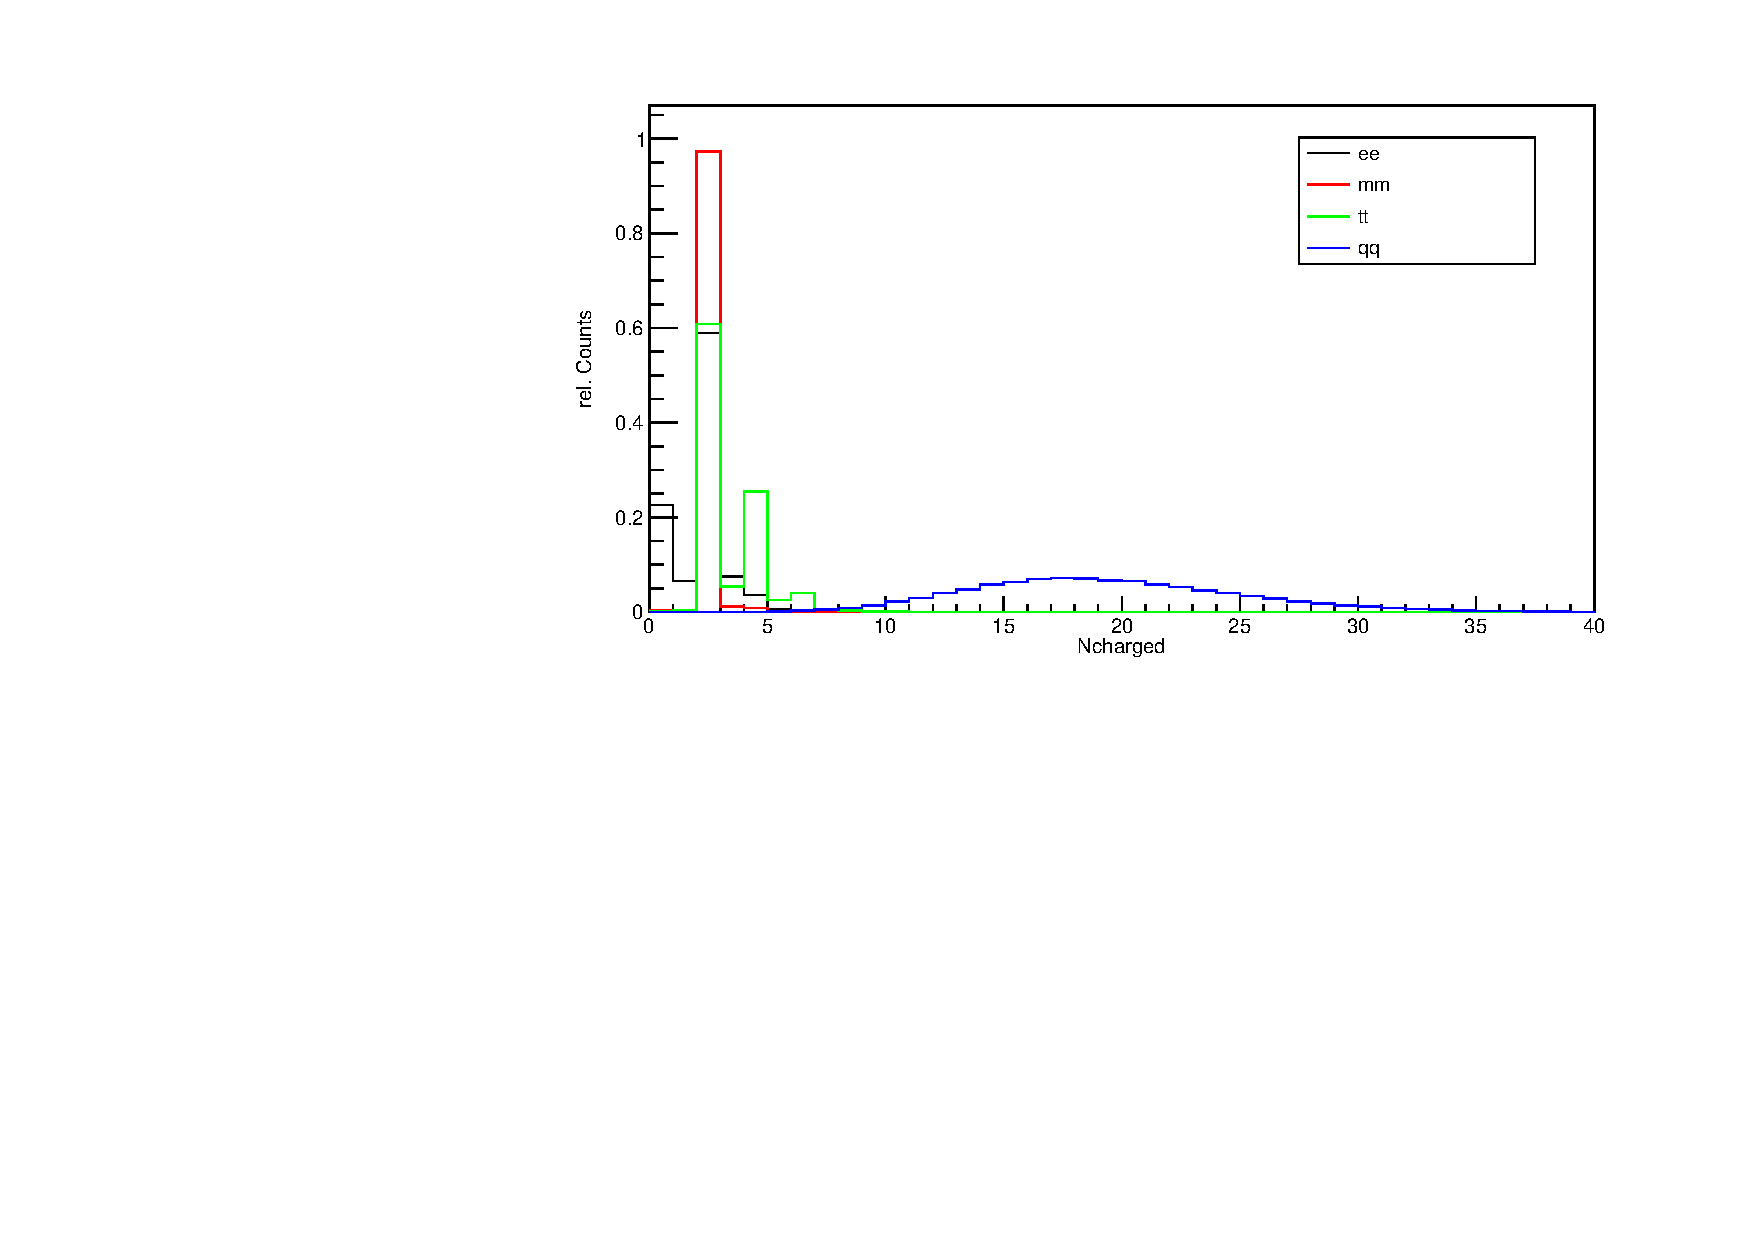
\includegraphics[width=\textwidth]{../img/dist_Ncharged.pdf}
  \caption{Monte-Carlo-Simulationen der vier Zerfallskanäle für die Anzahl der detektierten Spuren.}
  \label{img:dist_Ncharged}
\end{center}
\end{figure} 

\subsubsection*{Schnitte auf PCHARGED}
\begin{description}
\item[\Zmm:] Die Energie der Myonen ist im Spurdetektor gut messbar;
wir schneiden gegen \qq, \tt\ und einige \ee\ mit \emph{größer 75}.
\item[\Ztt:] Die Verteilung der Tauonen ist recht breit, trotzdem kann man mit \emph{größer~5}
gegen die Nulleinträge der \ee\ und \mm\ und mit \emph{kleiner 50} gegen \mm\ und einige \qq\ schneiden.
\end{description}


\begin{figure}[H]
\begin{center}
  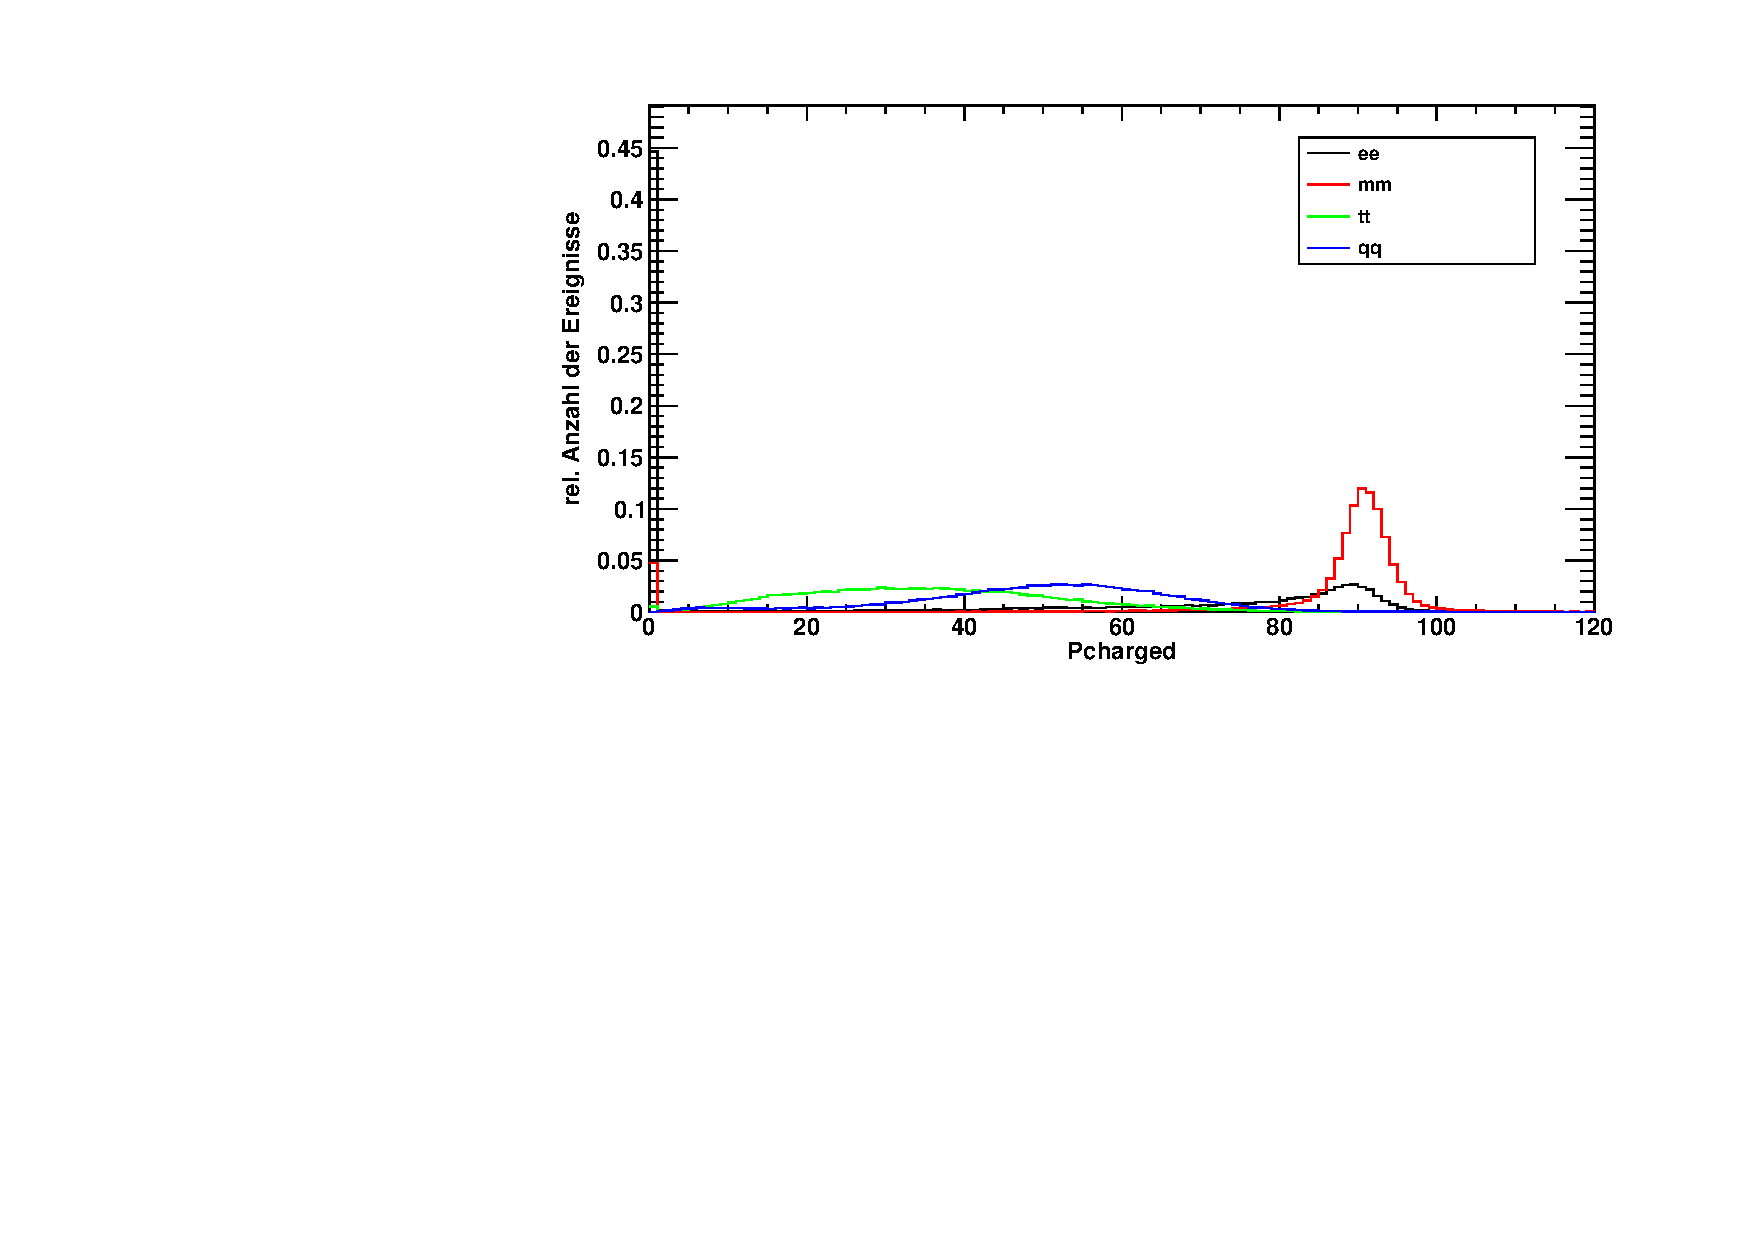
\includegraphics[width=\textwidth]{../img/dist_Pcharged.pdf}
 \caption{Monte-Carlo-Simulationen für die im Spurdetektor gemessene Energie.}
  \label{img:dist_Pcharged}
\end{center}
\end{figure} 

\subsubsection*{Schnitte auf E\_ECAL}
\begin{description}
\item[\Zee:] Im el. Kalorimeter können \ee-Ereignisse deutlich
gegen die anderen Zerfälle abgegrenzt werden.
Der Schnitt findet bei \emph{größer 75} statt.
\item[\Zmm:] Die Energie im el. Kalorimeter ist der einzige Parameter, mit dem \mm\ effektiv
von \ee\ getrennt werden können.
Der Schnitt findet bei \emph{kleiner 50} statt.
\item[\Ztt:] Gegen \mm\ wird mit \emph{größer 4} geschnitten, gegen Elektronen mit \emph{kleiner~70}.
\end{description}

\begin{figure}[H]
\begin{center}
  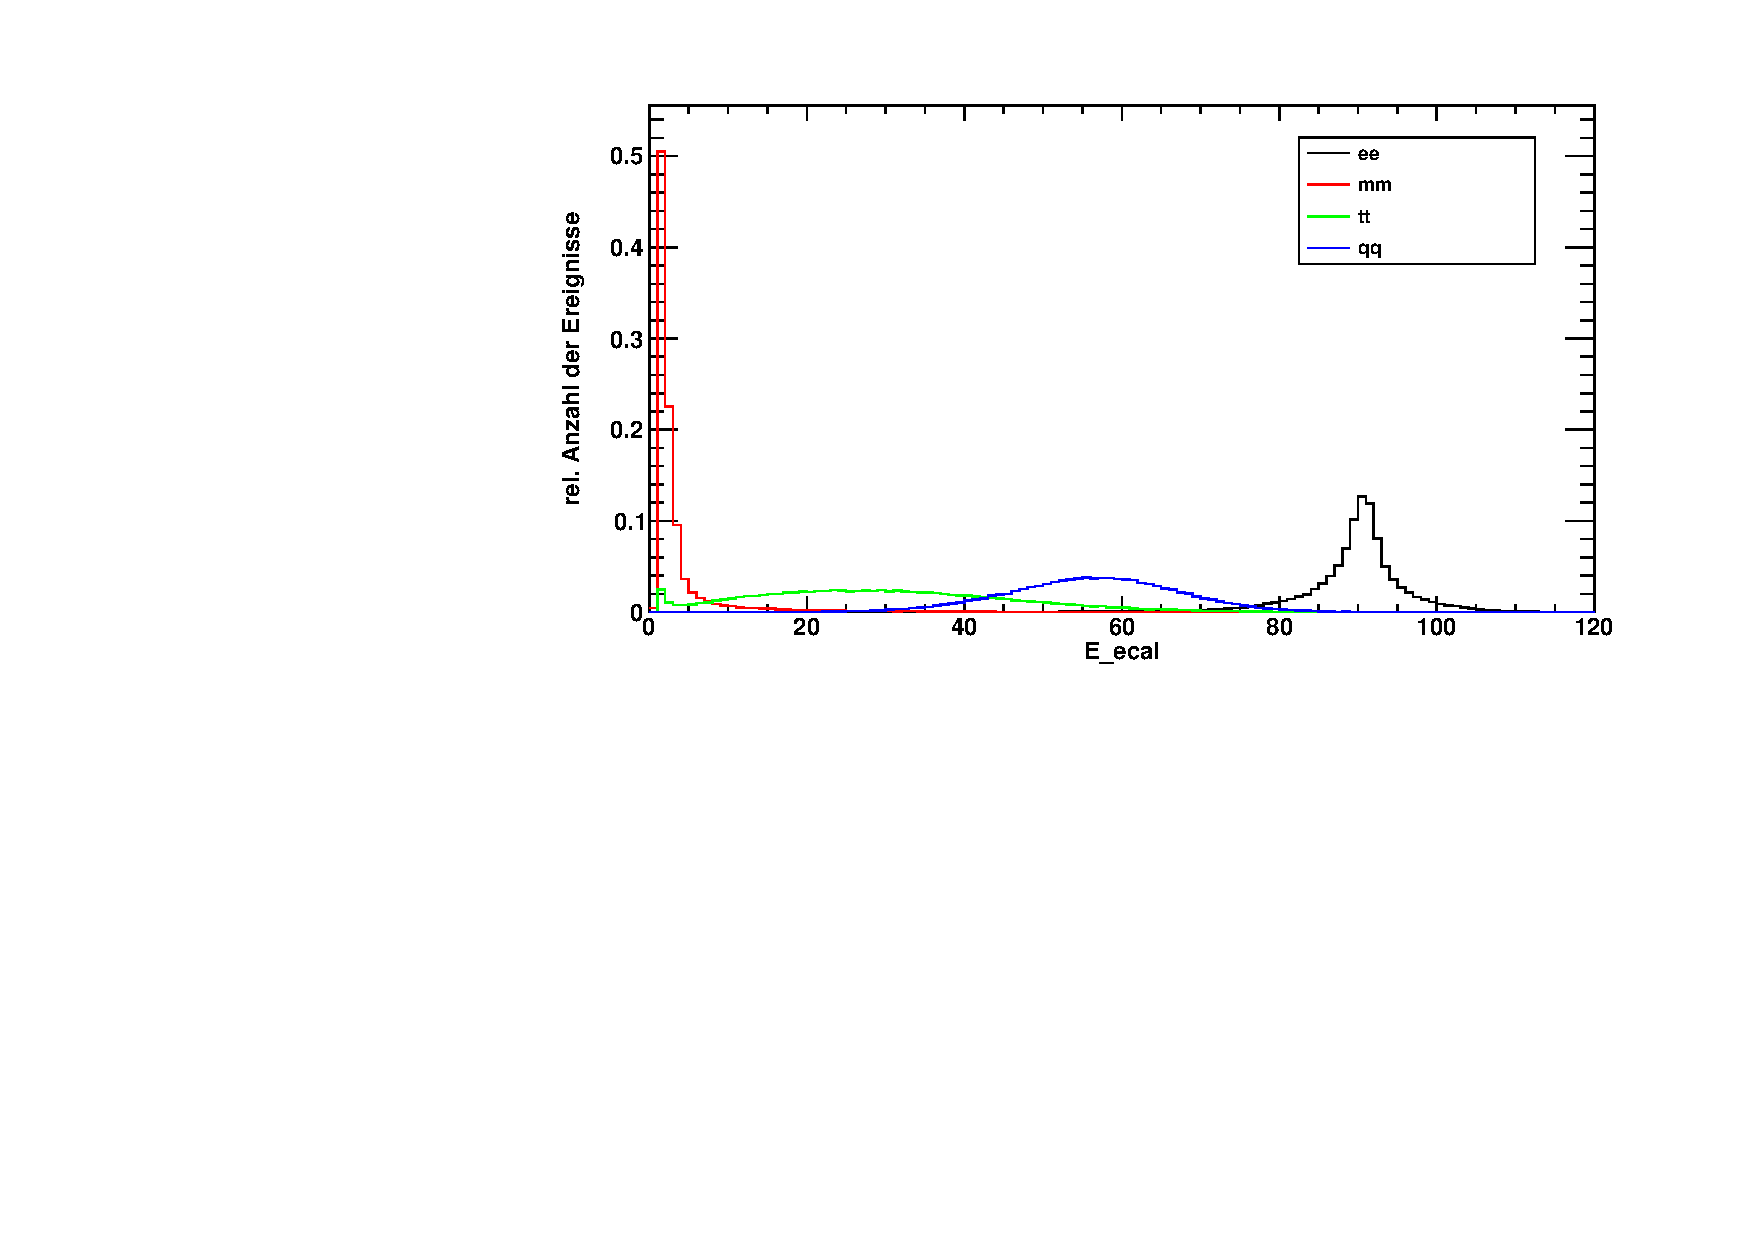
\includegraphics[width=\textwidth]{../img/dist_E_ecal.pdf}
 \caption{Monte-Carlo-Simulationen für die im elektromagnetischen Kalorimeter
 gemessene Energie.}
  \label{img:dist_E_ecal}
\end{center}
\end{figure} 

\subsubsection*{Schnitte auf E\_HCAL}
Im hadronischen Kalorimeter sind die vier Energiespektren nicht deutlich voneinander abgrenzbar,
daher werden hier keine Schnitte durchgeführt.

\begin{figure}[H]
\begin{center}
  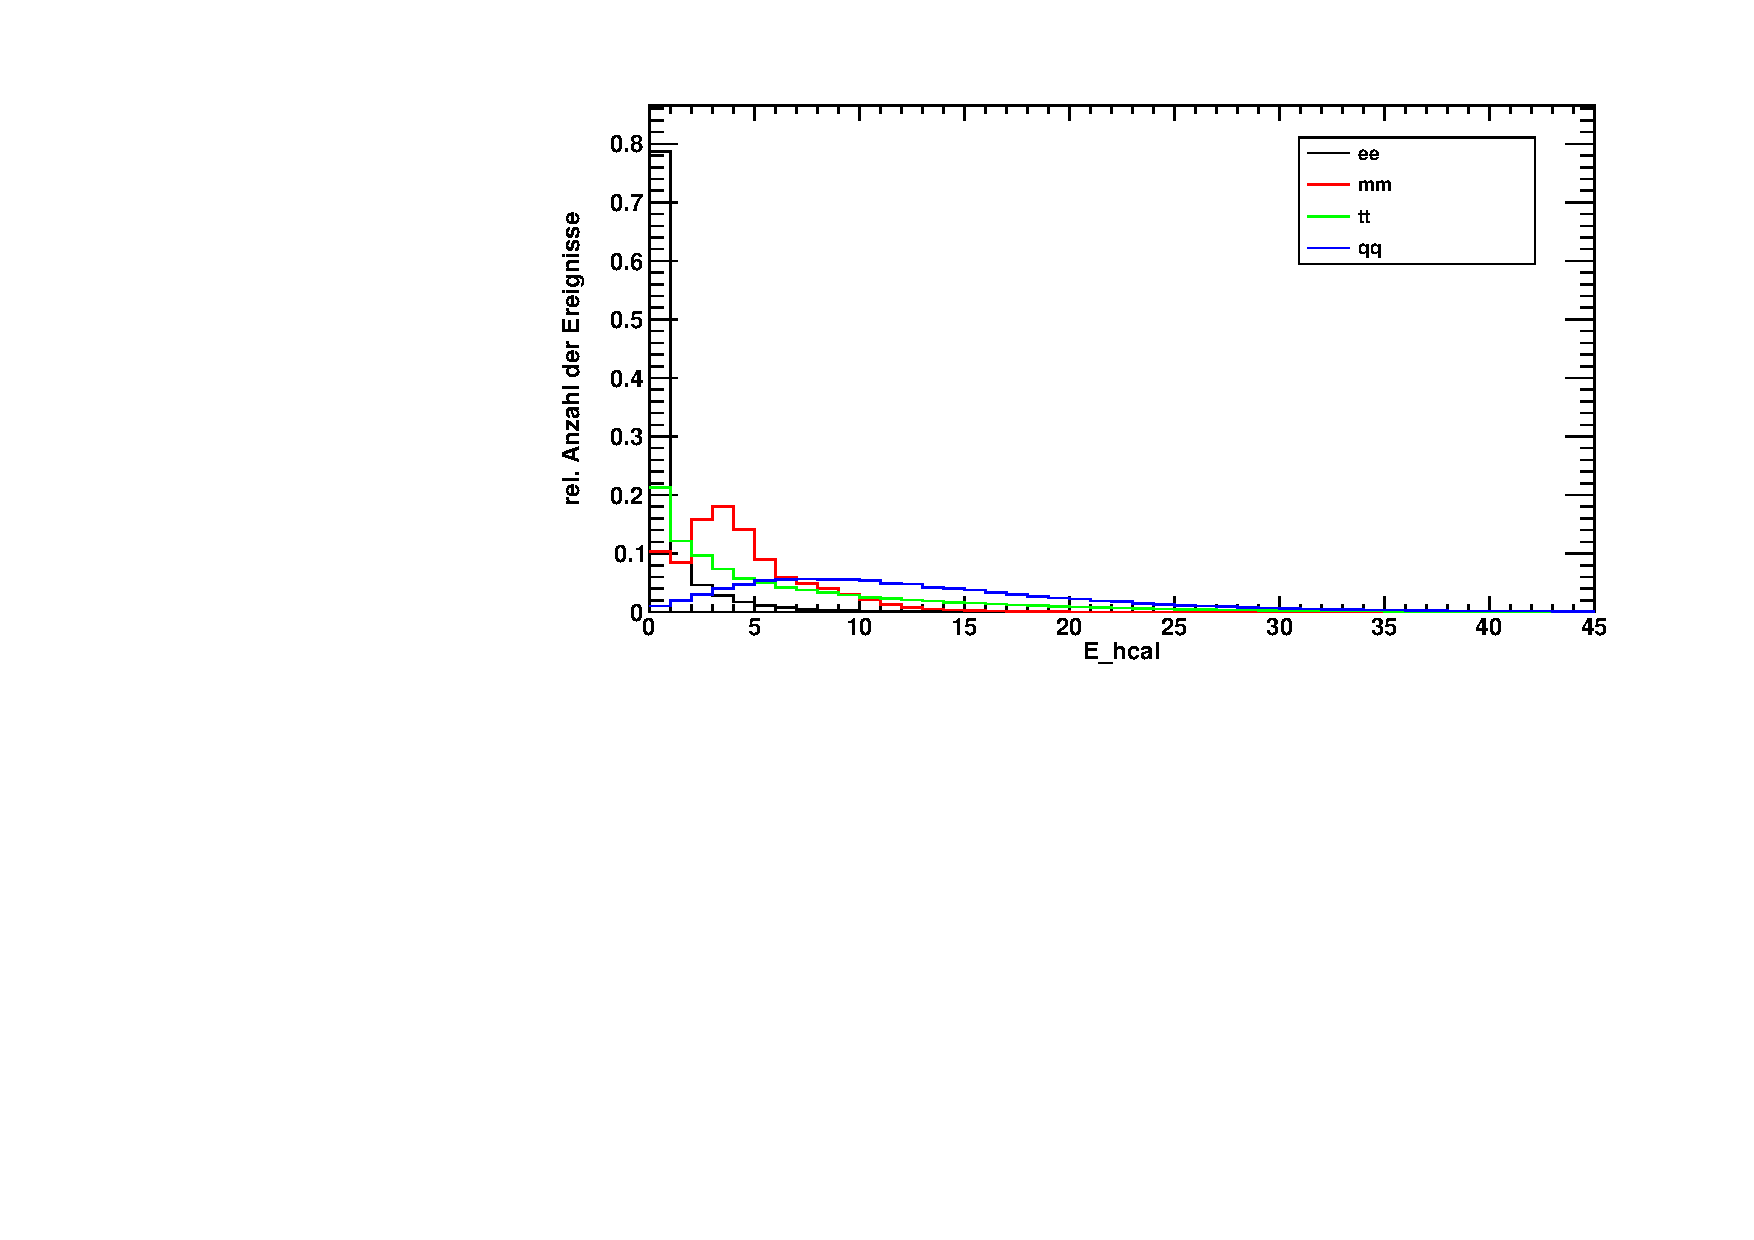
\includegraphics[width=\textwidth]{../img/dist_E_hcal.pdf}
 \caption{Monte-Carlo-Simulationen für die im hadronischen Kalorimeter
 gemessene Energie.}
  \label{img:dist_E_hcal}
\end{center}
\end{figure} 

\subsubsection*{Schnitte auf COS\_THET}
\begin{description}
\item[\Zee:] Um die \ee-Ereignisse abzuschneiden, die durch Bhabha-Streuung entstehen,
verlangen wir hier \emph{größer -0.9} und \emph{kleiner 0.9}.
\end{description}

\begin{figure}[H]
\begin{center}
  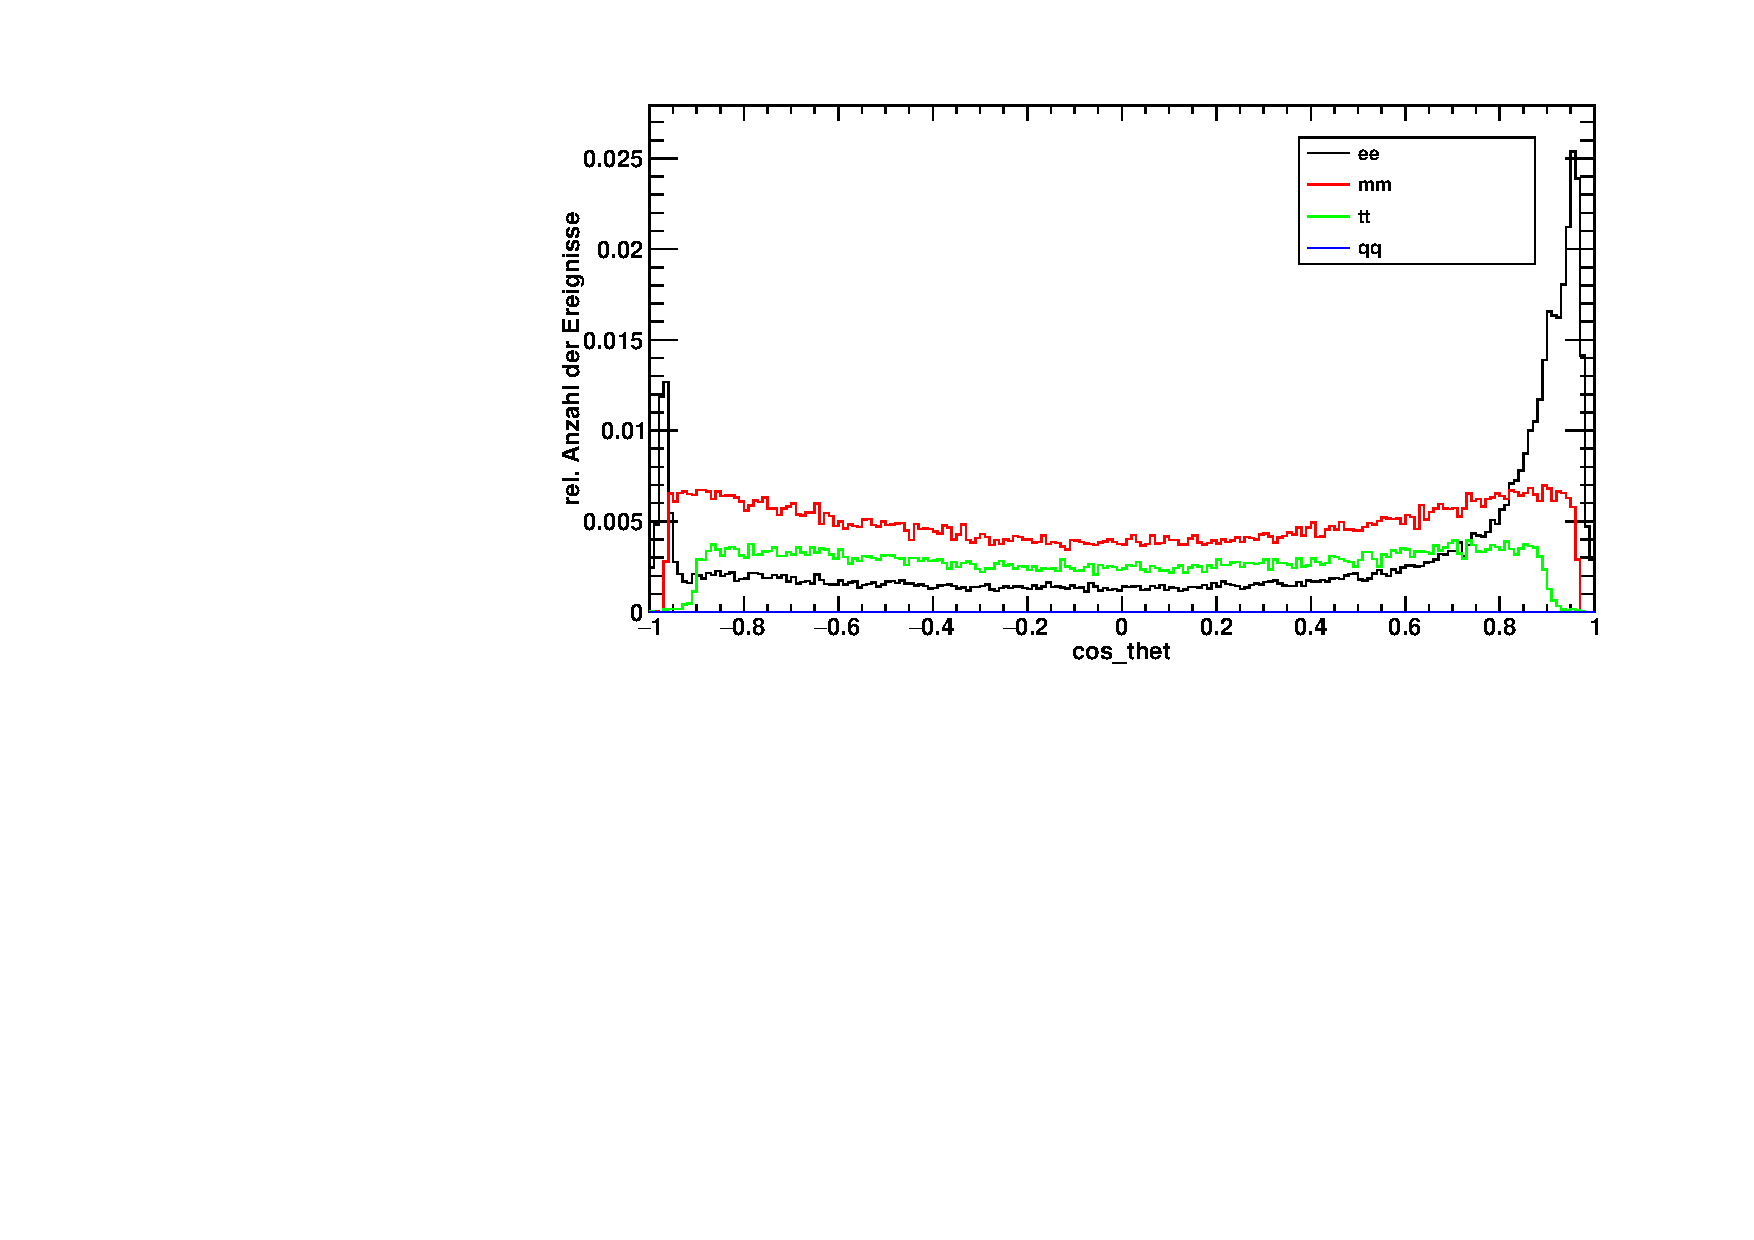
\includegraphics[width=\textwidth]{../img/dist_cos_thet.pdf}
 \caption{Monte-Carlo-Simulationen für die Polarwinkelverteilungen der positiven Leptonen.}
  \label{img:dist_cos_thet}
\end{center}
\end{figure} 

%TODO Formel Reinheiten
Die Reinheiten der Schnitte wurden mit folgender Formel bestimmt
\begin{equation}
  FORMEL
\end{equation}
und sind in \autoref{tab:reinheiten} aufgeführt.


\begin{table}[H]
    \caption{Berechnete Reinheit der Messdaten nach Anwendung der Schnitte aus \autoref{tab:schnitte}.}
    \begin{center}
        \begin{tabular}{|c|c|}
            \hline
   Zerfallskanal   	& Reinheit / \%	\\ \hline
   \Zee				& 99.9922		\\ \hline
   \Zmm				& 99.9871		\\ \hline
   \Ztt				& 99.7672		\\ \hline
   \Zqq				& 99.9936		\\ \hline

        \end{tabular}
    \end{center}
    \label{tab:reinheiten}
\end{table}

\subsection{Berechnung der Effizienzmatrix}
Werden die oben bestimmten Schnitte auf die Monte-Carlo-Daten angewendet, kann man die Effizienz $\bm{E}$ der Schnitte berechnen.
Die Effizienzmatrix gibt an, welcher Anteil der verschiedenen Ereignisse nach einem Schnitt noch vorhanden sind. Sie ist definiert als
\begin{equation}
    \bm{E}_{ij} = \frac{n_{ij}^\text{cut}}{n_i} \ \, .
\end{equation}
$i, j \in $ e$^+$e$^-$, \textmu$^+$\textmu$^-$, \texttau$^+$\texttau$^-$, q$^+$q$^-$ \\  %TODO format
Dabei bezeichnet $n_{ij}^\text{cut}$ die Anzahl der Ereignisse von Typ $i$ nach Schnitt von Typ $j$ und $n_i$ die gesamte Anzahl von Ereignissen
der Monte-Carlo-Simulation von Typ $i$.
Die Beziehung zwischen den Anzahlen von gemessenen Ereignissen nach Schnitt $\vec{M}$\footnote{"measurement"} und den echten Anzahlen
$\vec{T}$\footnote{"truth"} lautet durch die Definition der Effizienzmatrix $\bm{E}$:
\begin{equation}
    \label{eq:effmat:mtrel}
    \vec{M} = \bm{E} \vec{T}
\end{equation}
Die Effizienzmatrix unsere Schnitte ist in \autoref{tab:effmat:val} dargestellt.
\begin{table}[H]
\caption{Effizienzmatrix.}
\begin{center}
\begin{tabular}{|c|c|c|c|c|}
  \hline
  Schnitt$\backslash$MC-Daten & \ee & \mm & \tt & \qq \\ \hline
  \ee & 0.388233 & 0.000011 & 0.001995 & 0.000010 \\ \hline
  \mm & 0.000160 & 0.890762 & 0.003585 & 0.000000 \\ \hline
  \tt & 0.001791 & 0.004259 & 0.747406 & 0.002354 \\ \hline
  \qq & 0.000000 & 0.000000 & 0.001868 & 0.966965 \\ \hline
\end{tabular}
\end{center}
\label{tab:effmat:val}
\end{table}

Nun gilt es den Fehler der einzelnen Einträge der Effizienzmatrix zu bestimmen. Hierzu wird die Definition der Effizienz $\epsilon$ leicht geändert:
\begin{equation}
    \epsilon = \frac{p}{p+f}
\end{equation}
Die Anzahl der Ereignisse, die nach Schnitt noch da sind, wird mit $p$\footnote{"pass"} bezeichnet. Aus der totalen Anzahl $n$ der Ereignisse lässt
sich die Anzahl derjenigen Ereignisse $f$\footnote{"fail"} berechnen, die beim Schnitt wegfallen. Da $p$ und $f$ als poissonverteilt angenommen
werden können (bei hinreichenden Größen von $p$ und $f$), gilt für den Fehler der Effizienz mit Gauß'scher Fehlerfortpflanzung:
\begin{equation}
    s_\epsilon = \sqrt{\frac{f \cdot p}{ \left( f + p \right)^3}} \ \, .
\end{equation}
Mit der Definition von $\epsilon$ und $n$ kann man den Fehler zu der in der Literatur üblichen Form umformen:
\begin{equation}
    s_\epsilon = \sqrt{\frac{\epsilon (1-\epsilon)}{n}}
\end{equation}
Somit können nun die Fehler von den Einträge der Effizienzmatrix bestimmt werden (\autoref{tab:effmat:err}).
\begin{table}[H]
\caption{Fehler der Effizienzmatrix.}
\begin{center}
\begin{tabular}{|c|c|c|c|c|}
  \hline
  Schnitt$\backslash$MC-Daten & \ee & \mm & \tt & \qq \\ \hline
  \ee & 0.001591 & 0.000011 & 0.000159 & 0.000010 \\ \hline
  \mm & 0.000041 & 0.001015 & 0.000212 & 0.000000 \\ \hline
  \tt & 0.000138 & 0.000212 & 0.001544 & 0.000154 \\ \hline
  \qq & 0.000000 & 0.000000 & 0.000153 & 0.000569 \\ \hline
\end{tabular}
\end{center}
\label{tab:effmat:err}
\end{table}

\subsubsection{Berechnung der inversen Effizienzmatrix}
Wenn die Schnitte auf die echten Daten angewendet werden, sind nur die gemessenen Anzahlen von Ereignissen bekannt
(d.h. der $\vec{M}$-Vektor). Um auf die wahre Anzahl von Ereignissen rückzuschließen kann an \autoref{eq:effmat:mtrel}
von links die inverse Effizienzmatrix multipliziert werden:
\begin{equation}
    \vec{T} = \bm{E}^{-1} \vec{M}
\end{equation}
Die Inverse von \autoref{tab:effmat:val} ist in \autoref{tab:inveffmat:val} abgebildet.
\begin{table}[H]
\caption{Inverse Effizienzmatrix \bm{E}^{-1}.}
\begin{center}
\begin{tabular}{|c|c|c|c|c|}
  \hline
  Schnitt$\backslash$MC-Daten & \ee & \mm & \tt & \qq \\ \hline
  \ee & 2.575807 & 0.000002 & -0.006874 & -0.000010 \\ \hline
  \mm & -0.000438 & 1.122660 & -0.005384 & 0.000013 \\ \hline
  \tt & -0.006170 & -0.006398 & 1.338017 & -0.003257 \\ \hline
  \qq & 0.000012 & 0.000012 & -0.002585 & 1.034170 \\ \hline
\end{tabular}
\end{center}
\label{tab:inveffmat:val}
\end{table}

Den Fehler auf die Inverse einer Matrix ist nicht so einfach auszurechnen. Es wird ein numerisches Simulationsverfahren,
das \emph{toy-experiment}, verwendet: \\
Hierzu werden $N$\footnote{Für die Auswertung wurde $N=100000$ gesetzt.} Effizienzmatrizen $\bm{E}^k$ ($k=1 \ldots N$) erzeugt,
deren Einträge leicht modifiziert werden. Für jeden Eintrag $(\bm{E})_{ij}$ wird eine Zufallszahl $R_{ij}^k$
gewählt, die wie eine Gauß'sche Normalverteilung $\mathcal{N}(\mu, \sigma)$ mit Erwartungswert $\mu = 0$ und
Standardabweichung $\sigma = 1$ verteilt ist ($R \sim \mathcal{N}(0, 1)$). Der neue Eintrag $(\bm{E}^k)_{ij}$ wird nun folgendermaßen berechnet:
\begin{equation}
    (\bm{E}^k)_{ij} = (\bm{E})_{ij} + R_{ij}^k \cdot s_{(\bm{E})_{ij}}
\end{equation}
Die neuen Einträge sind also um die wahren Werte herum gaußverteilt. Nun wird die Inverse ${(\bm{E}^k})^{-1}$ jeder
Effizienzmatrix $\bm{E}^k$ erzeugt und
anschließend die Standardabweichung der einzelnen Einträge berechnet:
\begin{equation}
    s_{(\bm{E}^{-1})_{ij}} = \sqrt{\frac{1}{N-1} \sum_{i=1}^{N} \left((({\bm{E}^k)}^{-1})_{ij} - (\bm{E}^{-1})_{ij} \right)^2 }
\end{equation}
Die Standardabweichungen $s_{(\bm{E}^{-1})_{ij}}$ werden als Fehler auf die inverse Effizienzmatrix $\bm{E}^{-1}$ verwendet
(\autoref{tab:inveffmat:err}).
\begin{table}[H]
\caption{Fehler der inversen Effizienzmatrix, berechnet mit einem toy-experiment.}
\begin{center}
\begin{tabular}{|c|c|c|c|c|}
  \hline
  Schnitt$\backslash$MC-Daten & \ee & \mm & \tt & \qq \\ \hline
  \ee & 0.0023825 & 0.0000159 & 0.0004139 & 0.0000336 \\ \hline
  \mm & 0.0000607 & 0.0012753 & 0.0003189 & 0.0000012 \\ \hline
  \tt & 0.0002418 & 0.0003180 & 0.0027662 & 0.0002141 \\ \hline
  \qq & 0.0000007 & 0.0000012 & 0.0002127 & 0.0006094 \\ \hline
\end{tabular}
\end{center}
\label{tab:inveffmat:err}
\end{table}

\subsection{s-t-Kanal Trennung}
Wie in \autoref{subsub:theo:stchannel} beschrieben, besitzt die Bhabha-Streuung (\ee $\to$ \ee) einen s-Kanal (Annihilation)
und einen t-Kanal (Streuung). Da nur im s-Kanal ein reelles \Z -Boson entsteht, verfälschen die Ereignisse im t-Kanal die Anzahl
der \ee -Ereignisse. \\
Um den s-Kanal vom t-Kanal zu trennen, werden die echten Daten nach den verschiedenen Schwerpunktsenergieen $\sqrt{s}$ aufgeteilt und
der \ee -Schnitt angewendet. Es wird die Winkelabhängigkeit der Daten überprüft, da die Anzahl der \ee -Ereignisse
je nach Kanal eine unterschiedliche (vgl. \autoref{eq:stchannel:sigmas}) Abhängigkeit von $\cos \Theta$ besitzt. An den so erhaltenen Histogrammen wird
eine Kurvenanpassung mit
\begin{equation}
    \begin{split}
        & N(\cos \Theta) = s \cdot N_s(\cos \Theta ) + t \cdot N_t(\cos \Theta) \\
        & N_s(\cos \Theta) := \left( 1 + \cos^2 \Theta \right) \\
        & N_t (\cos \Theta) := \left( 1 - \cos \Theta \right)^{-2}
    \end{split}
\end{equation}
im Bereich von $-0.9 \leq \cos \Theta \leq 0.9$\footnote{Dies entspricht dem \ee -Schnitt.} durchgeführt. In \autoref{img:st:9123} sieht man
das Histogramm und den Fit der Daten mit einer Energie von \sE{91.23}. Die Graphen der anderen Schwerpunktsenergieen befinden sich in
\autoref{sub:app:st}.

\begin{figure}[H]
    \begin{center}
        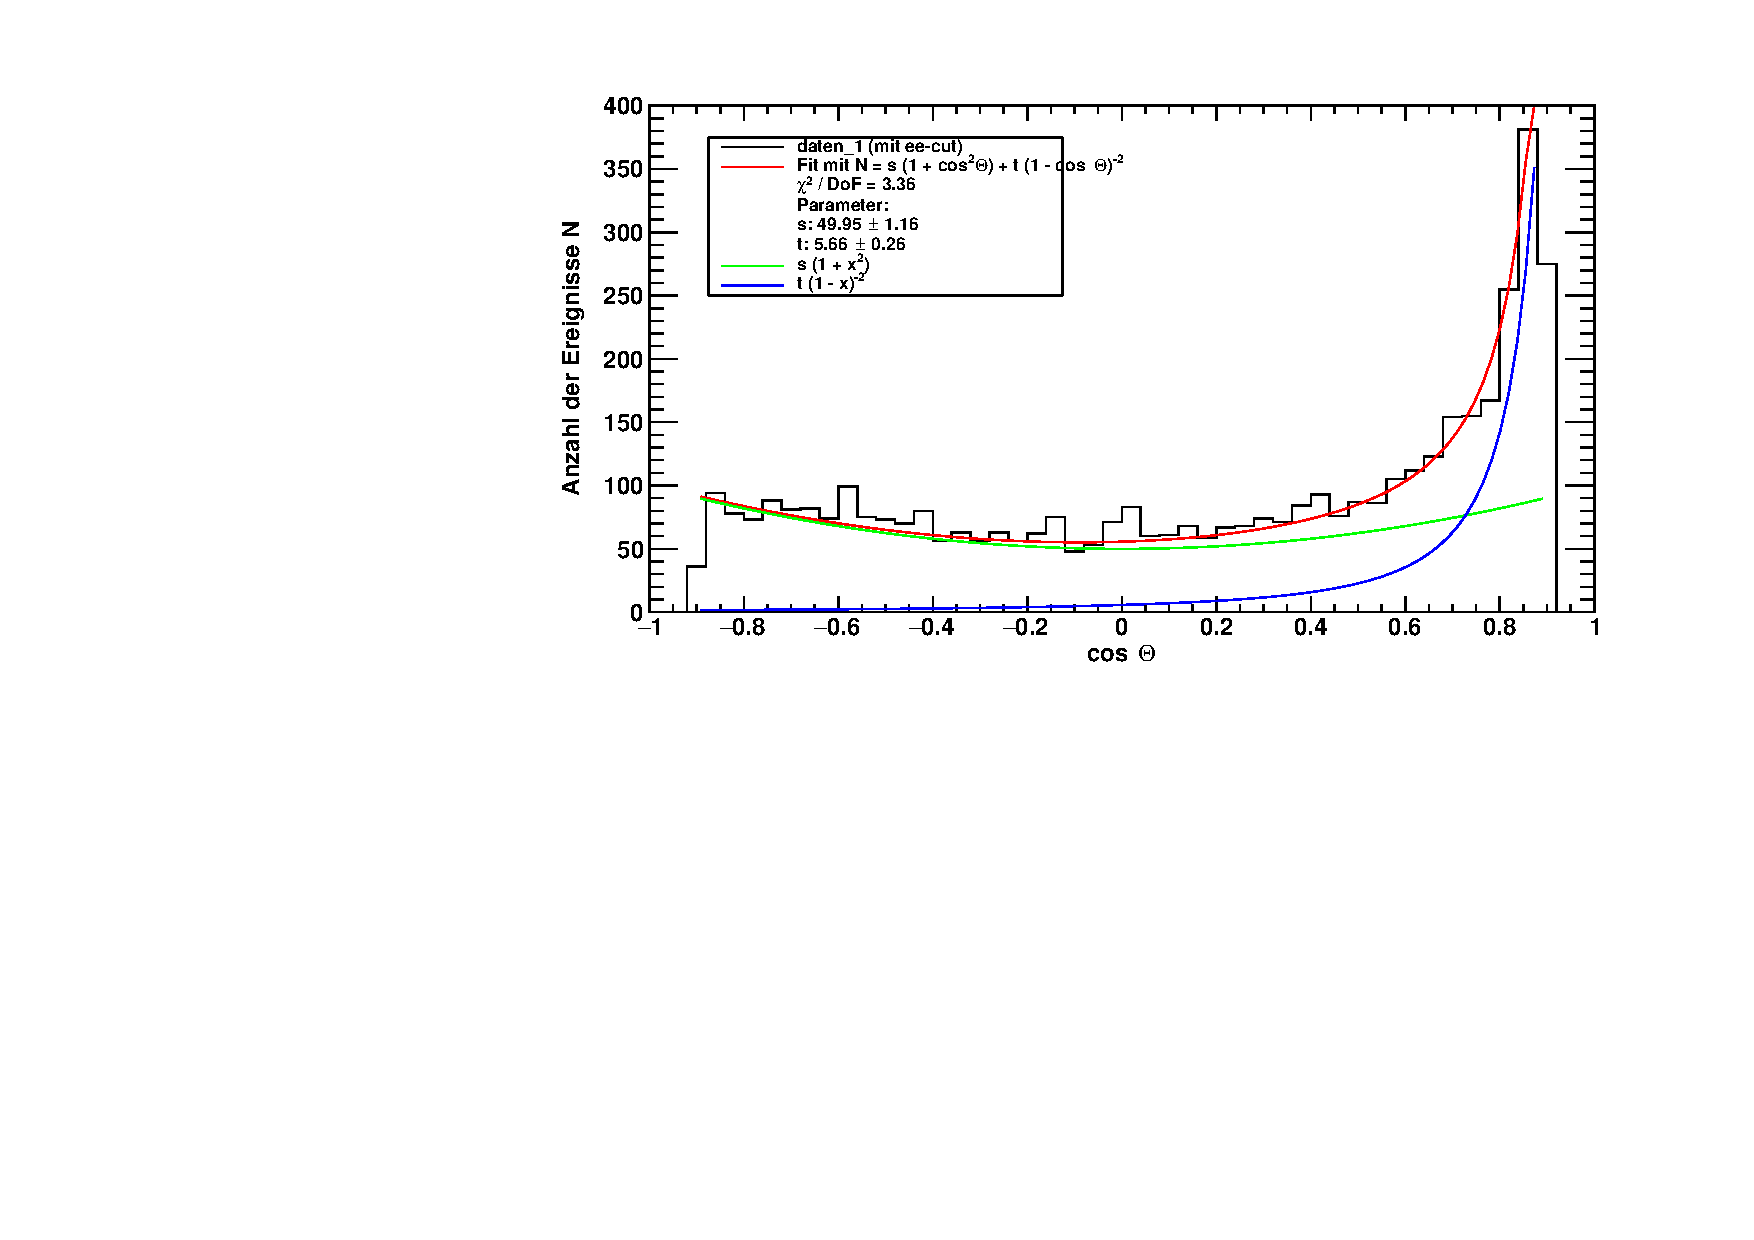
\includegraphics[width=\textwidth]{../img/s_t_fit_91-23.pdf}
        \caption{Winkelabhängigkeit der Ereignisse bei \sE{91.23} und Fit zur Bestimmung des s- und t-Anteils.}
        \label{img:st:9123}
    \end{center}
\end{figure}
Um die Anzahl $N_s^\text{tot}$ und $N_t^\text{tot}$ der s-Kanal bzw. t-Kanal Ereignisse zu erhalten, muss man
$s \cdot N_s(\cos \Theta)$ und $t \cdot N_t(\cos \Theta)$ einzeln integrieren. Dabei werden für die Parameter $s$ und $t$ die
gefitteten Werte benutzt. Die Fehlerfortpflanzung ist trivial, da die Integrale nicht von $s$ bzw. $t$ abhängen.
\begin{equation}
    \begin{split}
        & N_s^\text{tot} = s \cdot \int_{-0.9}^{0.9} \left( 1 + \cos^2 \Theta \right) \difd (\cos \Theta) \\
        & N_t^\text{tot} = t \cdot \int_{-0.9}^{0.9} \left( 1 - \cos \Theta \right)^{-2} \difd (\cos \Theta)
    \end{split}
\end{equation}
Nun kann der s-t-Korrekturterm $c_{\text{st}}$ bestimmt werden:
\begin{equation}
    c_{\text{st}} = \frac{N_s^\text{tot}}{N_s^\text{tot} + N_t^\text{tot}}, \qquad
    s_{c_{\text{st}}} = c_{\text{st}} \cdot \sqrt{ \left( \frac{s_{N_s^\text{tot}}}{N_s^\text{tot}} \right)^2 +
    \frac{s_{N_s^\text{tot}}^2 + s_{N_t^\text{tot}}^2}{ \left( N_s^\text{tot} + N_t^\text{tot} \right)^2 } }
\end{equation}
Wird $c_{\text{st}}$ mit einer gemessenen Anzahl von \ee -Ereignissen multipliziert, erhält man den die Anzahl der s-Kanal Ereignisse.
Die Korrekturwerte für die verschiedenen Schwerpunktsenergieen sind in \autoref{tab:st:corrs} aufgelistet.
\begin{table}[H]
\caption{Korrekturfaktoren $c_{\text{st}}$ der s-t-Kanal Trennung für verschiedene Schwerpunktsenergien.}
\begin{center}
\begin{tabular}{|c|c|c|}
  \hline
  $\sqrt{s}$ / GeV & $c_{\text{st}}$ & $s_{c_{\text{st}}}$ \\ \hline
  88.48 & 0.15 & 0.03 \\ \hline
  89.47 & 0.38 & 0.05 \\ \hline
  90.23 & 0.51 & 0.05 \\ \hline
  91.23 & 0.68 & 0.02 \\ \hline
  91.97 & 0.74 & 0.06 \\ \hline
  92.97 & 0.49 & 0.07 \\ \hline
  93.72 & 0.44 & 0.06 \\ \hline
\end{tabular}
\end{center}
\label{tab:st:corrs}
\end{table}


\subsection{Berechnung der Wirkungsquerschnitte}
Nun können die Wirkungsquerschnitte der verschiedenen Prozesse ausgerechnet werden. Hierzu werden die echten Daten nach den verschiedenen
Schwerpunktsenergieen aufgeteilt und die verschiedenen Schnitte angewendet. Die Anzahl der Ereignisse, die nach den verschiedenen Schnitten
noch übrig sind, werden im $\vec{M}$-Vektor gespeichert. Durch linksseitige Multiplikation mit der inversen Effizienzmatrix $\bm{E}^{-1}$
wird der $\vec{T}$-Vektor berechnet.
\begin{equation}
    T_i = \left( \bm{E}^{-1} \vec{M} \right)_i = \sum_j (\bm{E}^{-1})_{ij} \cdot M_j
\end{equation}
Da die Einträge $M_i$ des $\vec{M}$-Vektors Ergebnisse eines Zähl-Experiment sind, sind sie poissonverteilt:
\begin{equation}
    s_{M_i} = \sqrt{M_i}
\end{equation}
Es folgt für den Fehler auf $T_i$:
\begin{equation}
    s_{T_i} = \sqrt{\sum_j \left( (\bm{E}^{-1})_{ij} \cdot M_j \right)^2 \cdot
    \left( \left( \frac{s_{(\bm{E}^{-1})_{ij}}}{(\bm{E}^{-1})_{ij}} \right)^2 + \left( \frac{\sqrt{M_j}}{M_j} \right)^2 \right) }
\end{equation}
Für Anzahl der \ee -Ereignisse muss noch die s-t-Korrektur durchgeführt werden:
\begin{equation}
    T_\text{\ee}' = c_\text{st} \cdot T_\text{\ee}, \qquad
    s_{T_\text{\ee}'} = T_\text{\ee} \cdot \sqrt{ \left( \frac{s_{T_\text{\ee}}}{T_\text{\ee}} \right)^2 + \left( \frac{s_{c_\text{st}}}{c_\text{st}} \right)^2 }
\end{equation}
Die Wirkungsquerschnitte lassen sich nun mit
\begin{equation}
    \sigma_i = \frac{T_i}{L} + c_{\text{beami}, i}, \qquad
    s_{\sigma_i} = \frac{T_i}{L} \cdot \sqrt{ \left( \frac{s_{T_i}}{T_i} \right)^2 + \left( \frac{s_L^\text{stat}}{L} \right) }
\end{equation}
ausrechnen. Dabei ist $L$ die über die Messzeit integrierte Luminosität aus \autoref{tab:lums}
und $c_{\text{beam}, i}$ die Strahlungskorrektur aus \autoref{tab:beamcorrs}.

\subsection{Auswertung der Wirkungsquerschnitte}
Die Wirkungsquerschnitte der verschiedenen Zerfallskanäle werden nun gegen die Schwerpunktsenergie $\sqrt{s}$ aufgetragen und mit einer 
relativistischen Breit-Wigner Funktion (\autoref{eq:sigma:fermion}) gefittet (\autoref{img:crosssection:ee} bis \autoref{img:crosssection:qq}).
\begin{equation}
    \sigma_i(s) = \frac{12 \pi}{M_\text{Z}^2} \cdot \frac{s \Gamma_j \Gamma_i}{ \left( s - M_\text{Z}^2 + s^2 \Gamma_\text{Z}^2 / M_\text{Z}^2 \right) }
\end{equation}
Die freien Parameter sind die Masse $M_\text{Z}$ des \Z-Bosons, die totale Breite $\Gamma_\text{Z}$ und 
die Partialbreiten $\Gamma_i$ und $\Gamma_j$. Eigentlich sollte $\Gamma_j$ immer die elektronische Breite $\Gamma_\text{e}$ sein, jedoch 
kann dies nicht mehr gefittet werden, da die beiden partiellen Zerfallsbreiten beide freie Parameter sind, die direkt miteinander multipliziert 
werden. Für die Wirkungsquerschnitte der leptonischen Zerfallskanäle wird deshalb Leptonenuniversalität angenommen und der Faktor $\Gamma_j \Gamma_i$ 
vereinfacht sich zu $\Gamma_i^2$. \\
Für den hadronischen Wirkungsquerschnitt ist die Situation ein bisschen anders, da hier keine Leptonenuniversalität angenommen werden kann. 
Da der gefittete Wert von $\Gamma_\text{e}$ nicht gut mit dem Literaturwert übereinstimmt (ausführliche Diskussion in \autoref{subsub:partWidth}), 
wird $\Gamma_i$ auf den gefitteten Wert von $\Gamma_\text{\textmu}$ fixiert.

\begin{figure}[H]
    \begin{center}
        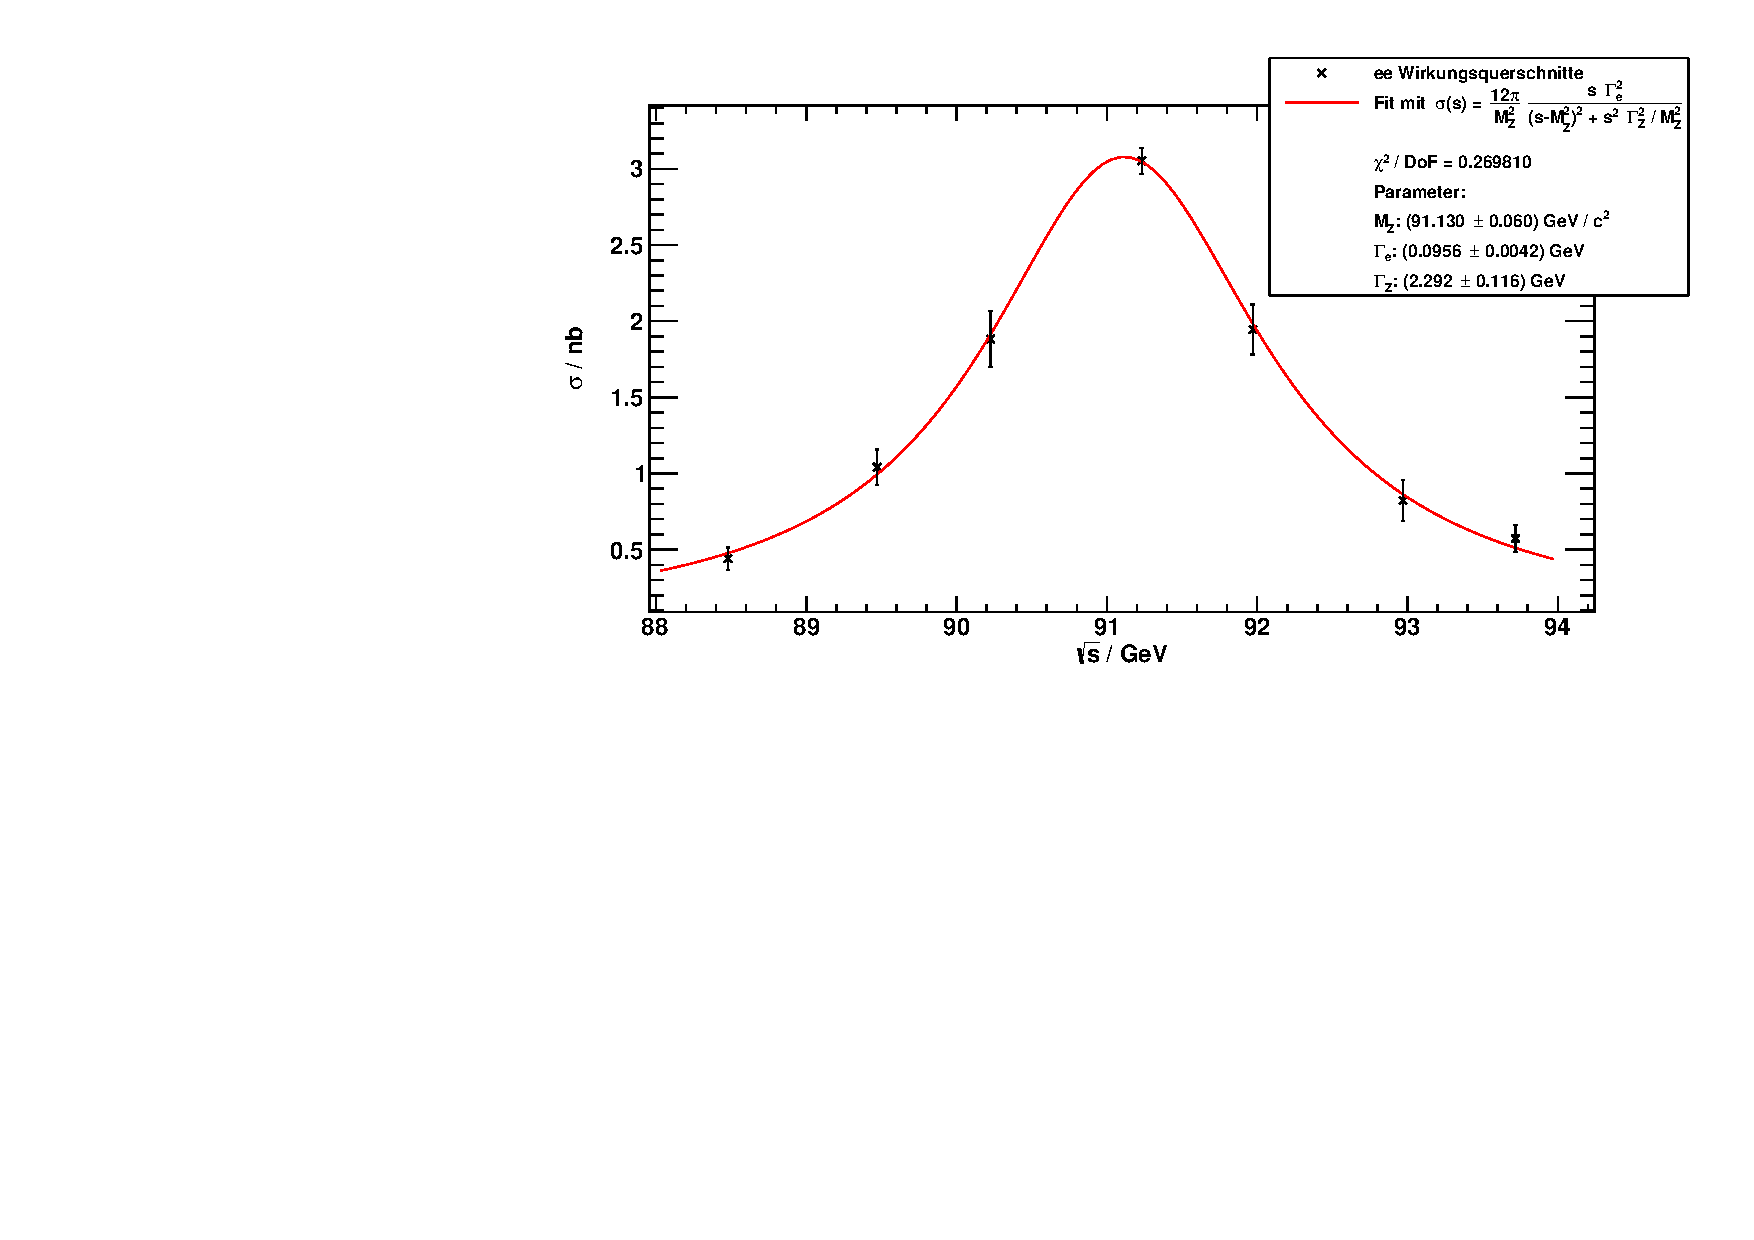
\includegraphics[width=\textwidth]{../img/crosssections_ee.pdf}
        \caption{Wirkungsquerschnitt für \ee $\to$ \ee.}
        \label{img:crosssection:ee}
    \end{center}
\end{figure}

\begin{figure}[H]
    \begin{center}
        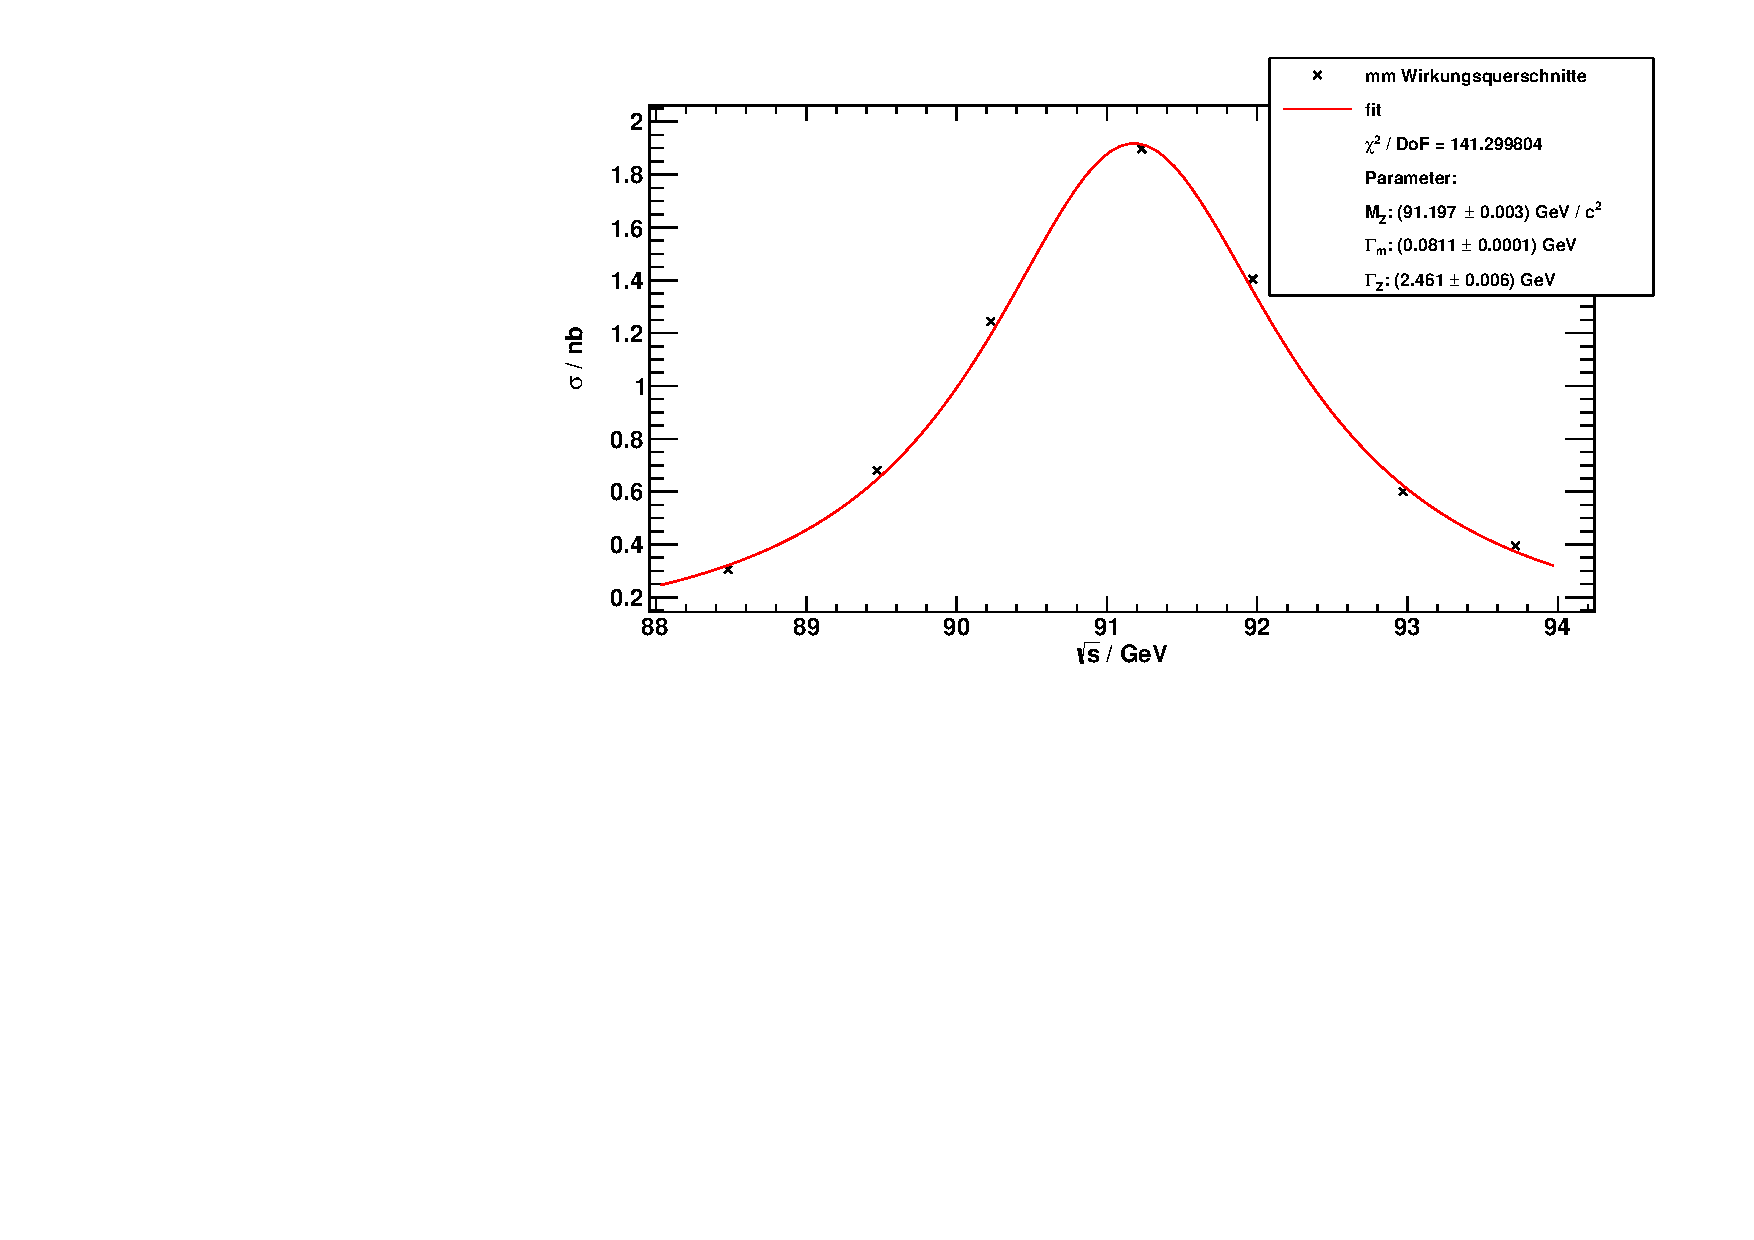
\includegraphics[width=\textwidth]{../img/crosssections_mm.pdf}
        \caption{Wirkungsquerschnitt für \ee $\to$ \mm.}
        \label{img:crosssection:mm}
    \end{center}
\end{figure}

\begin{figure}[H]
    \begin{center}
        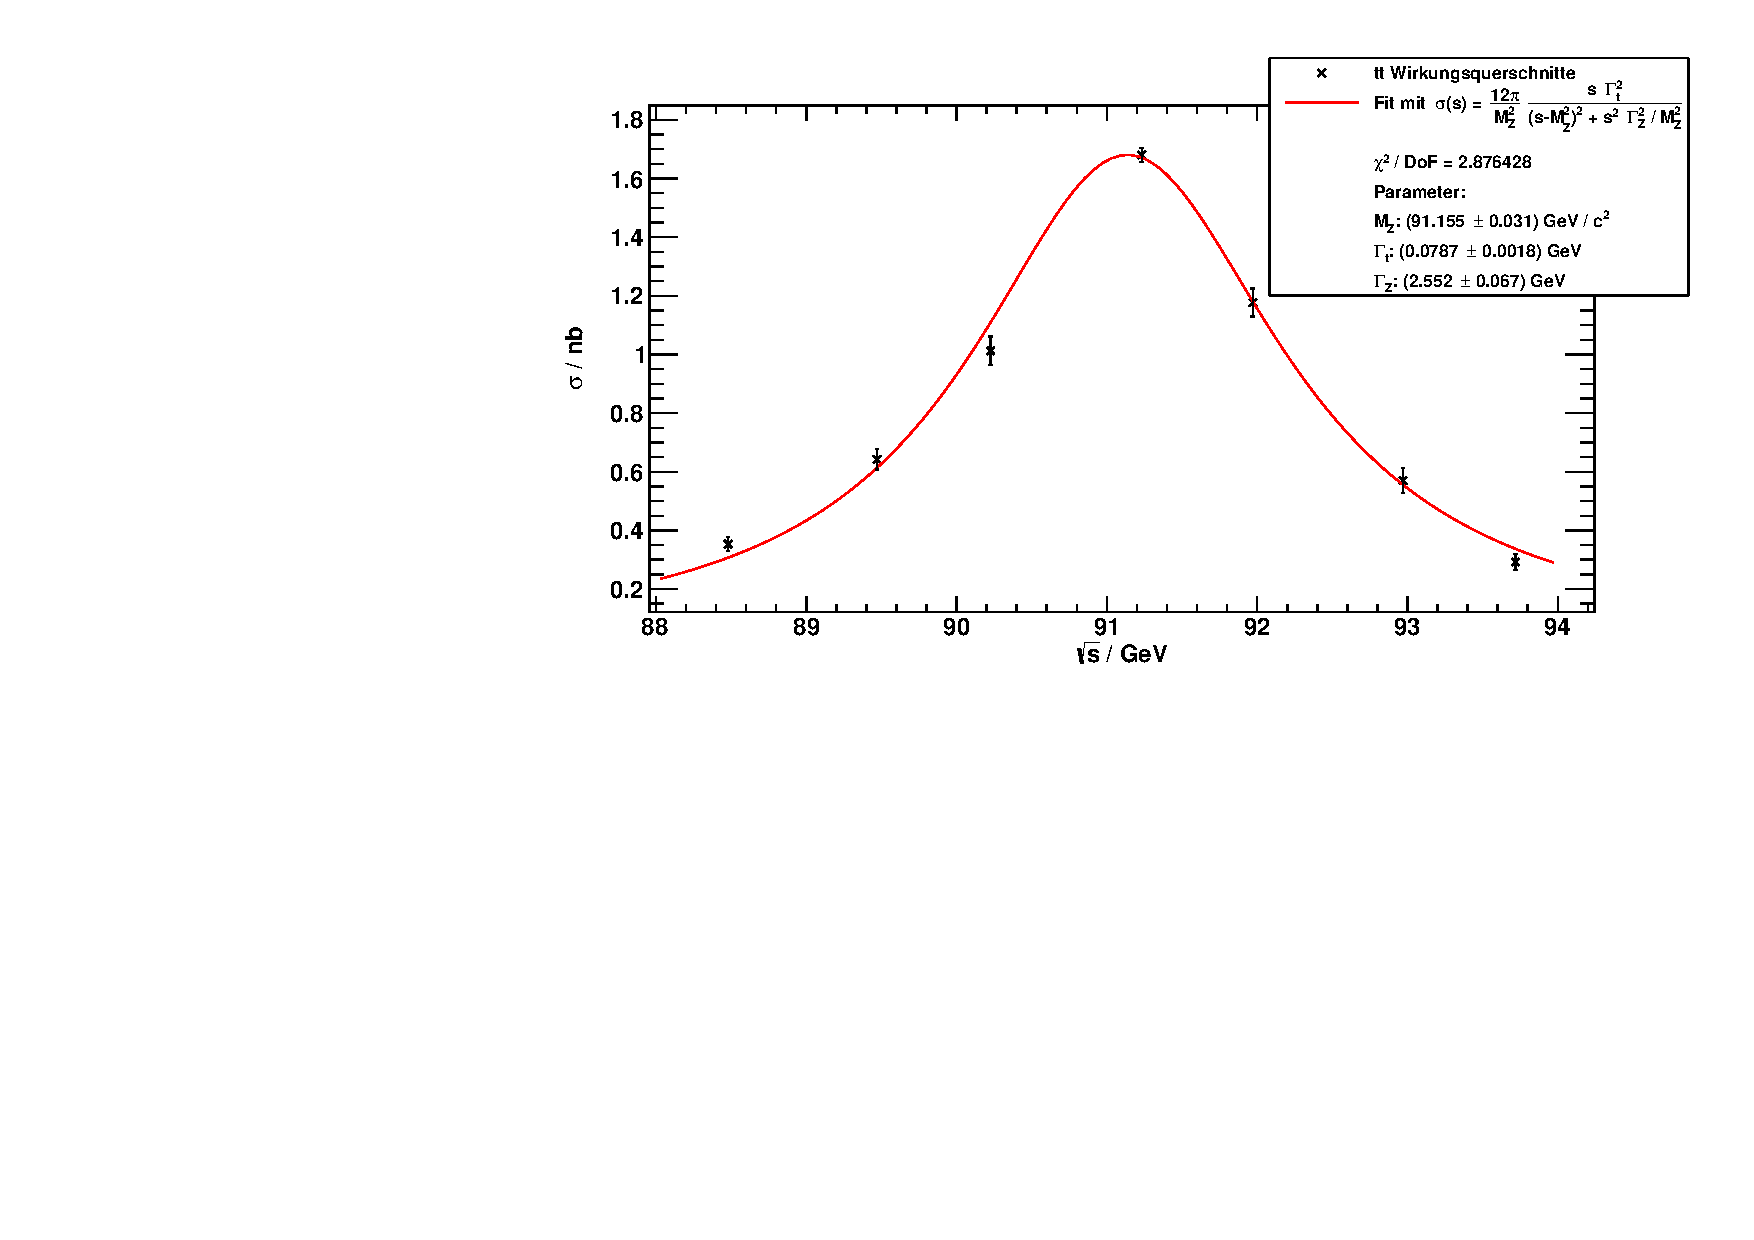
\includegraphics[width=\textwidth]{../img/crosssections_tt.pdf}
        \caption{Wirkungsquerschnitt für \ee $\to$ \tt.}
        \label{img:crosssection:tt}
    \end{center}
\end{figure}

\begin{figure}[H]
    \begin{center}
        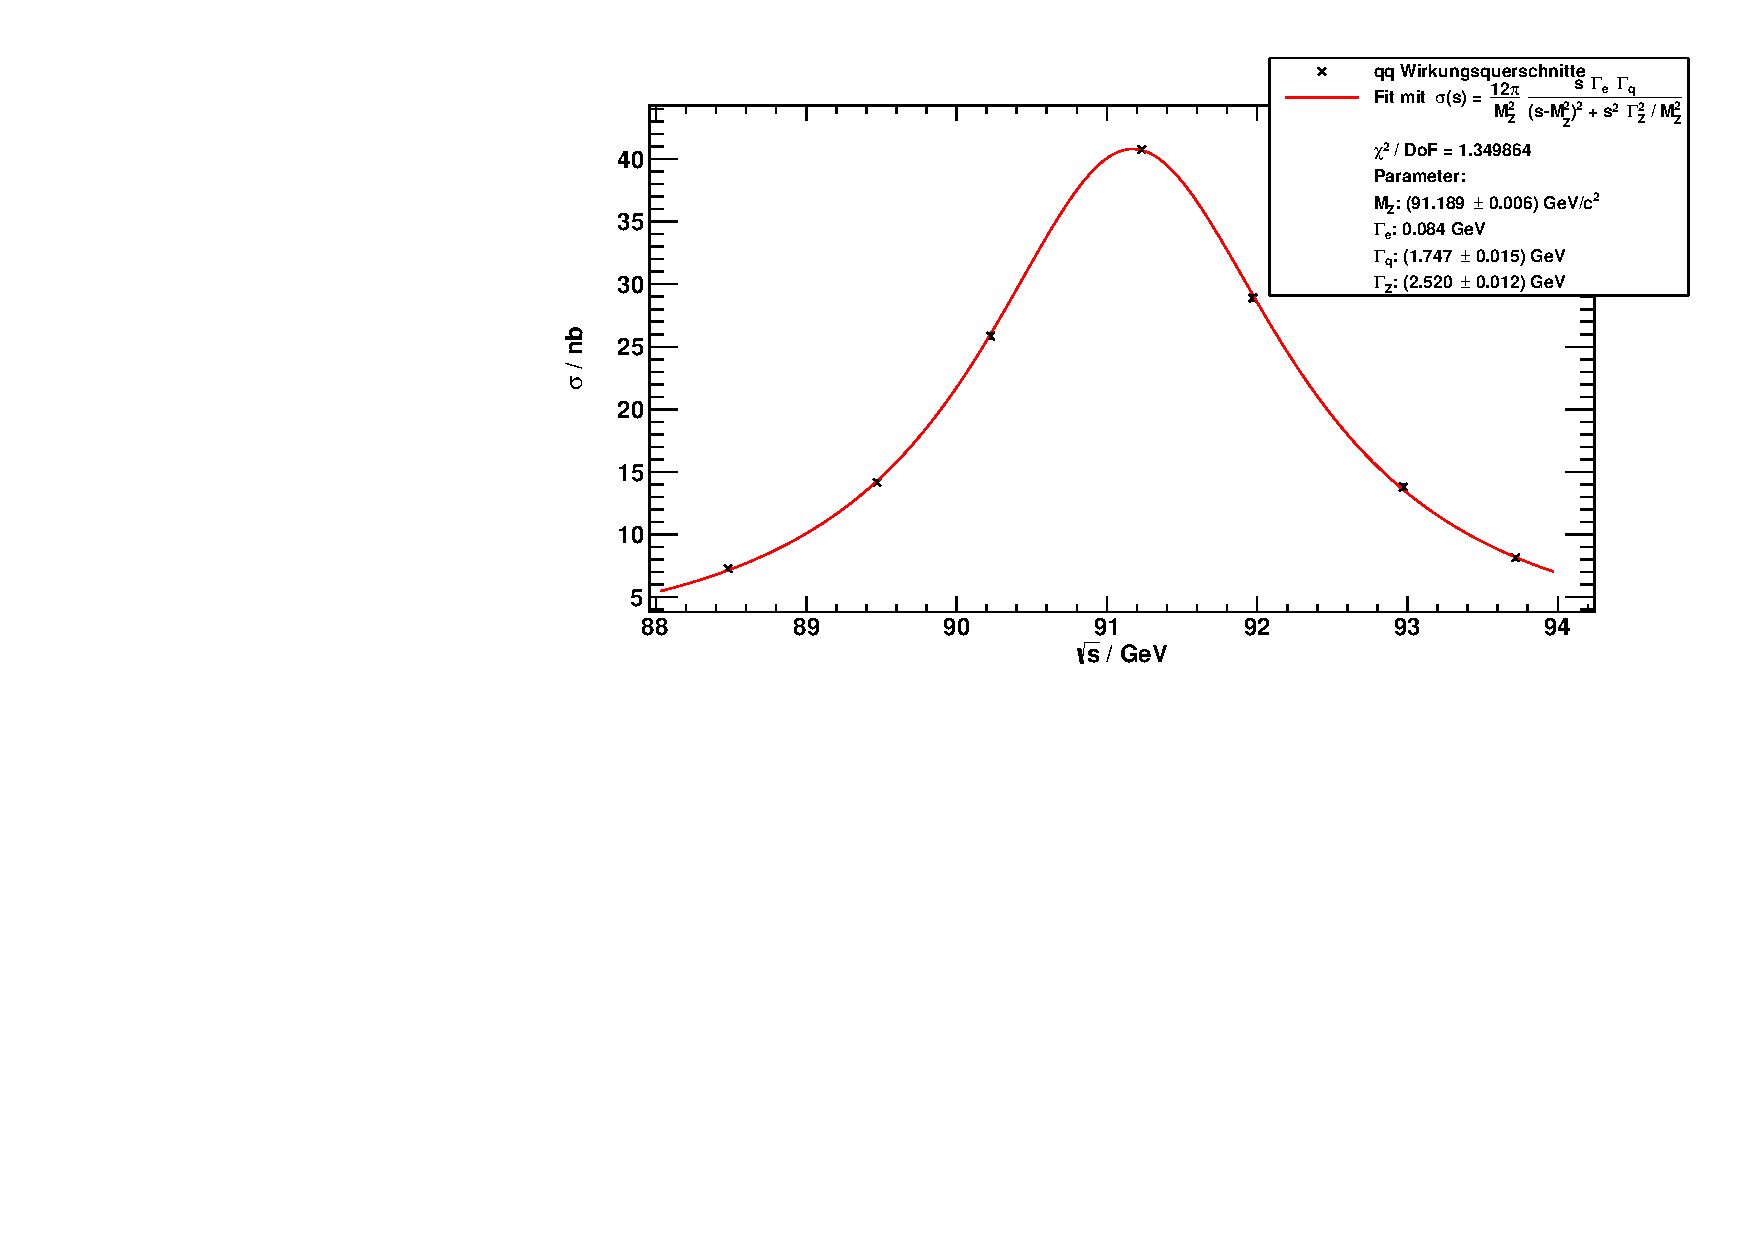
\includegraphics[width=\textwidth]{../img/crosssections_qq.pdf}
        \caption{Wirkungsquerschnitt für \ee $\to$ \qq.}
        \label{img:crosssection:qq}
    \end{center}
\end{figure}

\subsubsection{\Z-Masse}
Die durch die verschiedenen Zerfallskanäle bestimmten Massen des \Z-Bosons
und ihr gewichteter Mittelwert sind in \autoref{tab:mass} aufgelistet.
Alle Ergebnisse stimmen innerhalb ihrer Fehlergrenzen mit dem Literaturwert \cite{pdg} überein.

\begin{equation}
    M_\text{Z}^\text{Lit.} = (91.1876 \pm 0.0021)\,\text{GeV}
\end{equation}
\begin{table}[H]
\caption{Durch Fits bestimmte Masse des \Z-Bosons und gewichtetes Mittel.}
\begin{center}
\begin{tabular}{|c|c|c|}
  \hline
  Zerfallskanal & $M_\text{Z}$ / GeV & $s_{M_\text{Z}}$ / GeV \\ \hline
  \ee & 91.170 & 0.064 \\ \hline
  \mm & 91.194 & 0.028 \\ \hline
  \tt & 91.155 & 0.031 \\ \hline
  \qq & 91.189 & 0.006 \\ \hline
  gew. Mittel & 91.188 & 0.006 \\ \hline
\end{tabular}
\end{center}
\label{tab:mass}
\end{table}

\subsubsection{Totale Zerfallsbreite}
In \autoref{tab:gamma:total} befinden sich die Fitergebnisse für die totale Zerfallsbreite $\Gamma_\text{Z}$
und der gewichtete Mittelwert.
Die Übereinstimmungen mit dem Literaturwert
\begin{equation}
    \Gamma_\text{Z}^\text{Lit.} = (2.4952 \pm 0.0023)\,\text{GeV}
\end{equation}
sind im 1-\textsigma- und im 2-\textsigma-Intervall.
\begin{table}[H]
\caption{Durch Fits bestimmte totale Zerfallsbreite des \Z-Bosons und gewichtetes Mittel.}
\begin{center}
\begin{tabular}{|c|c|c|}
  \hline
  Zerfallskanal & $\Gamma_\text{Z}$ / GeV & $s_{\Gamma_\text{Z}}$ / GeV \\ \hline
  \ee & 2.355 & 0.113 \\ \hline
  \mm & 2.508 & 0.052 \\ \hline
  \tt & 2.560 & 0.067 \\ \hline
  \qq & 2.520 & 0.012 \\ \hline
  gew. Mittel & 2.518 & 0.012 \\ \hline
\end{tabular}
\end{center}
\label{tab:gamma:total}
\end{table}


\subsubsection{Partielle Zerfallsbreiten}
\label{subsub:partWidth}
Die Ergebnisse für die partiellen Zerfallsbreiten des \Z-Bosons befinden sich in \autoref{tab:gamma:part}.

Der Literaturwert für den elektronischen Zerfall liegt etwas mehr als 3 Standardabweichungen vom Ergebnis entfernt.
Die Ursache dafür könnte eine ungenaue s-t-Kanal-Trennung sein:
Wenn der Beitrag des t-Kanals bei der Trennung unterschätzt wird,
also nicht alle Teilchen der Bhabha-Streuung aus den Messdaten entfernt werden,
erhält man einen größeren Wirkungsquerschnitt des Prozesses und damit eine zu hohe Partialbreite.

Die myonische Partialbreite stimmt innerhalb ihrer Standardabweichung mit dem Literaturwert überein.

Das Ergebnis für die Tauonen schließt den Literaturwert innerhalb des 3-\textsigma-Intervalls ein.
Der Grund für die große Abweichung könnte die komplexe Signatur der \texttau-Ereignisse sein,
die die Wahl der Schnittparameter und die Identifikation der Ereignisse in den Messergebnissen schwierig macht.

Das Ergebnis für die hadronische Partialbreite liegt fast drei Standardabweichungen über dem Literaturwert.
Grund dafür ist der zu niedrige Wert der myonischen Partialbreite, der beim Fit verwendet wurde.

Aus den oben genannten Gründen kann die Leptonenuniversalität nur innerhalb des 4-\textsigma-Intervalls
bestätigt werden.

\begin{table}[H]
\caption{Durch Fits bestimmte partielle Zerfallsbreiten des \Z-Bosons.}
\begin{center}
\begin{tabular}{|c|c|c|}
  \hline
  Zerfallskanal $i$ & $\Gamma_i$ / GeV & $s_{\Gamma_i}$ / GeV \\ \hline
  \ee & 0.0971 & 0.0041 \\ \hline
  \mm & 0.0825 & 0.0015 \\ \hline
  \tt & 0.0790 & 0.0018 \\ \hline
  \qq & 1.7793 & 0.0153 \\ \hline
\end{tabular}
\end{center}
\label{tab:gamma:part}
\end{table}


\subsubsection{Anzahl leichter Neutrinogenerationen}
Die unsichtbare Zerfallsbreite $\Gamma_\text{inv.}$ ist die
Differenz von gemittelter Gesamtbreite und den Partialbreiten:
\begin{equation}
  \Gamma_\text{inv.}=\overline{\Gamma_\text{Z}}-\Gamma_\text{q}-\Gamma_\text{e}-\Gamma_\text{\textmu}-\Gamma_\text{\texttau}
  =(480 \pm 20)\,\text{GeV}
\end{equation}
Mit der oben berechneten theoretischen Zerfallsbreite für den Zerfall in Neutrino und Antineutrino
\begin{equation}
  \Gamma_\nu=165.841\,\text{MeV}
\end{equation}
erhält man für die Anzahl leichter Neutrinogenerationen
(unter der Annahme, dass die gesamte unsichtbare Zerfallsbreite durch Neutrinos verursacht wird)
\begin{equation}
  n=\frac{\Gamma_\text{inv.}}{\Gamma_\nu}=2.89 \pm 0.12 \ \, .
\end{equation}
Dieses Ergebnis passt in das Standardmodell mit seinen drei Neutrinogenerationen.

\subsection{Vorwärts-Rückwärts-Asymmetrie}
Um die Vorwärts-Rückwärts-Asymmetrie der myonischen Endzustände zu bestimmen,
erfolgt ein Fit an die Messdaten, die mit den Parametern für Myonen geschnitten wurden.
Die Fitfunktion lautet dabei
\begin{equation}
  N(\cos(\Theta))=\text{F}_1 \left (1+\cos^2(\Theta) \right) + 2 \text{F}_2\cos(\Theta)
\end{equation}
Da der erste Teil der Fitfunktion symmetrisch zur y-Achse ist,
ist die Information über die Asymmetrie im Fitparameter F$_2$ enthalten.
Der Fit liefert ein Ergebnis von
\begin{equation}
  \text{F}_2=-0.9 \pm 0.9 \ \, .
\end{equation}
Die Daten enthalten also keine signifikante Asymmetrie.
Für eine Aussage wären hier mehr Messpunkte notwendig,
um den Fehler auf die Fitparameter zu reduzieren und die feine Asymmetrie abzubilden.

\begin{figure}[H]
\begin{center}
  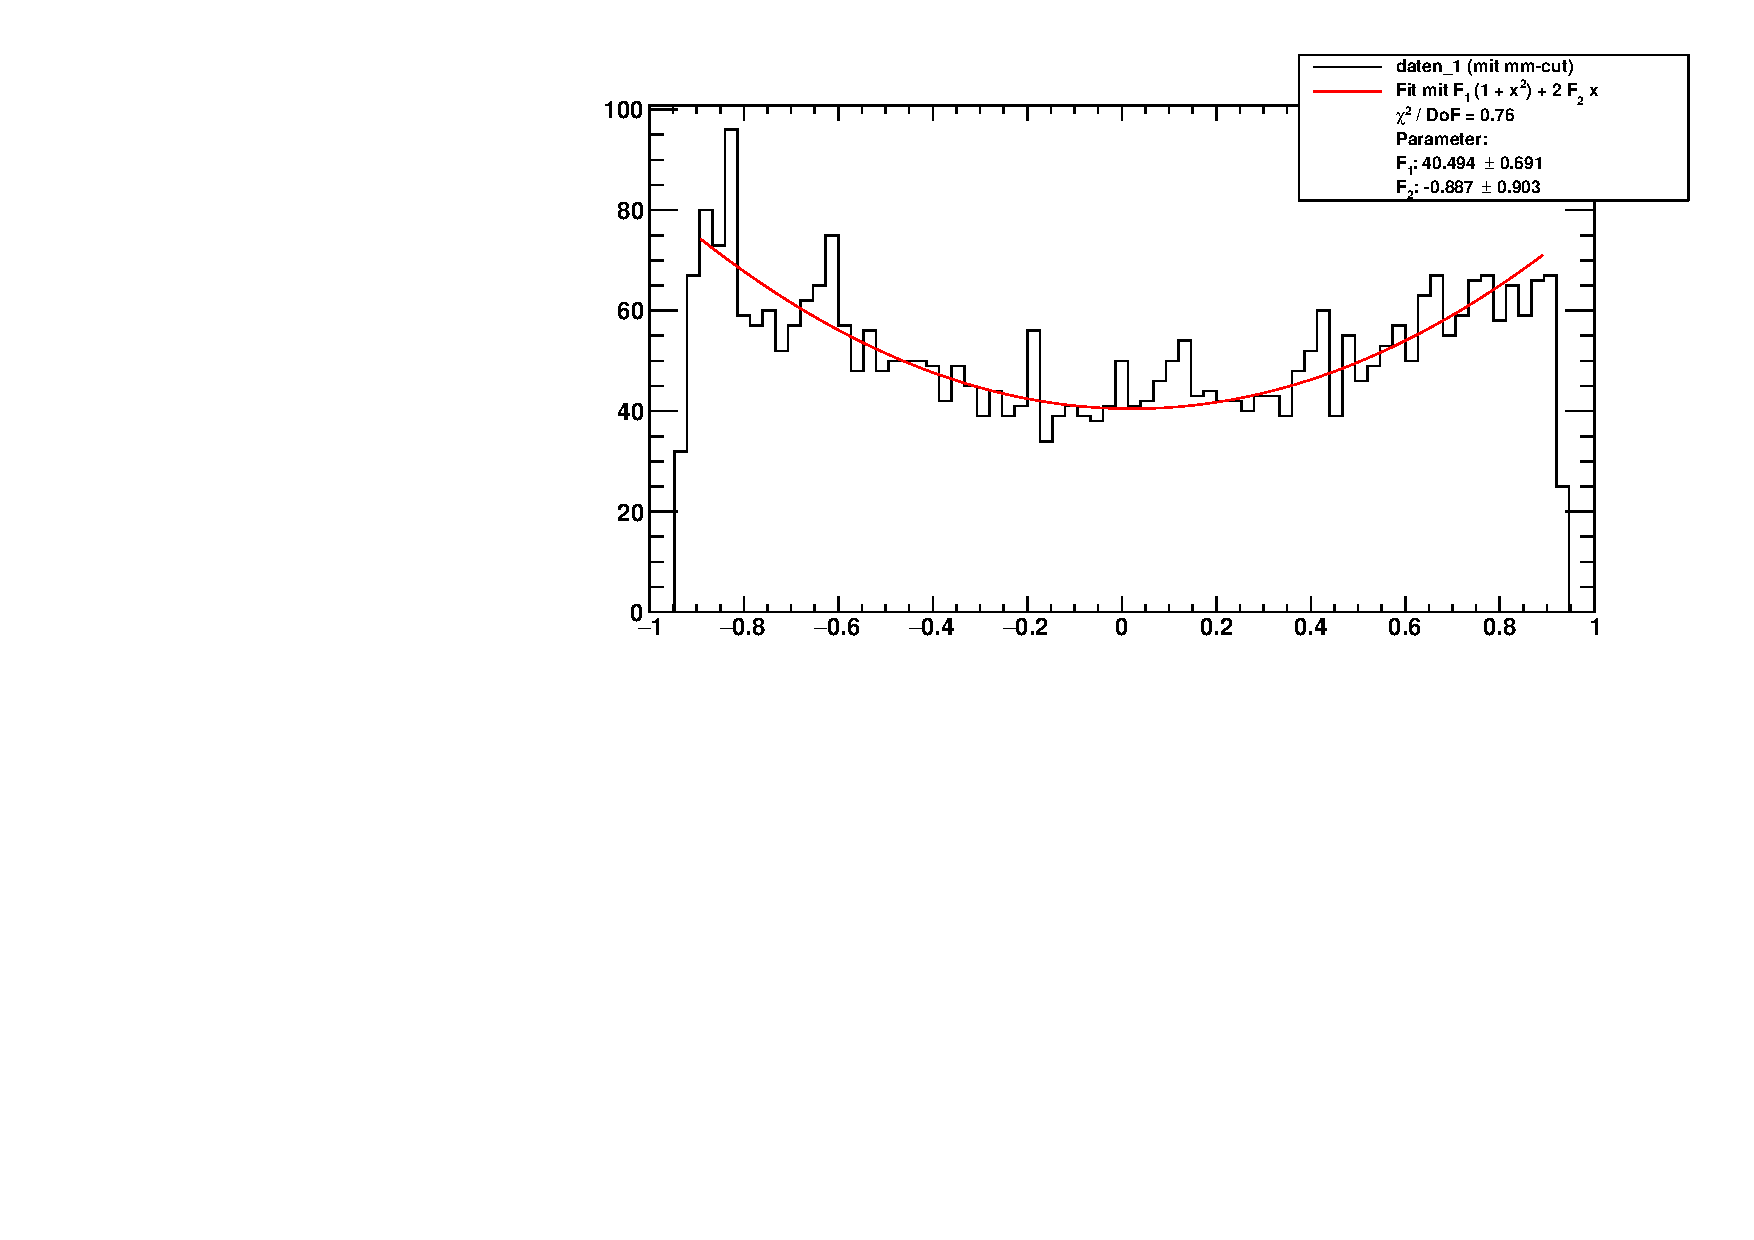
\includegraphics[width=\textwidth]{../img/FBA_91-23223.pdf}
  \caption{Polarwinkelverteilung der Myonen und Fit zur Bestimmung der Vorwärts-Rückwärts-Asymmetrie.}
  \label{img:FBA}
\end{center}
\end{figure}

